% -------------------- CONFIGURAÇÕES --------------------
% Básico:
\documentclass[
    article,
	12pt,				% tamanho da fonte
	%openright,			% capítulos começam em pág ímpar
	oneside,			% para impressão em recto e verso. Oposto a oneside
	a4paper,			% tamanho do papel. 
	english,			% idioma adicional para hifenização
	brazil,				% o último idioma é o principal do documento
	hyperref = {colorlinks, citecolor=c1d, linkcolor=c2d, urlcolor=c3d, colorlinks}
	]{abntex2}
\usepackage[T1]{fontenc}		% selecao de codigos de fonte.
\usepackage[utf8]{inputenc}		% codificacao do texto do documento
\usepackage{times} % fonte

% Layout:
\usepackage[left=3cm,right=2cm,bottom=2cm,top=3cm]{geometry} % definir margens
\setlength{\parskip}{\baselineskip} % espaço vertical pós parágrafo
\usepackage[bottom]{footmisc} % fixar footnote na parte de baixo da página

% definir contagem do TOC
\usepackage{chngcntr}
\counterwithin{section}{chapter}
\AtBeginDocument{\addtocontents{toc}{\changetocdepth{1}}}

% Cores:
\usepackage{xcolor}
\makeatletter % criar paletta "Dark2" do RColorBrewer (pacote do R)
\newcounter{j}
\@for\i:={1B9E77, D95F02, 7570B3, E7298A, 66A61E, E6AB02, A6761D, 666666}\do{
    \stepcounter{j}
    \definecolor{c\arabic{j}}{HTML}{\i}
    \colorlet{c\arabic{j}d}{c\arabic{j}!60!gray}}
\makeatother

% Gráficos:
\usepackage{graphicx}
\usepackage{tikz} 
\usetikzlibrary{positioning, shapes.geometric, backgrounds, chains, arrows.meta}

% Referências:
\usepackage[backend=biber, style=apa]{biblatex} 
\usepackage{csquotes} % requerimento do biblatex

% Matemática
\usepackage{amsmath}
\usepackage{amssymb}
\usepackage{multicol}
\usepackage{mathtools}
\usepackage{bm} % símbolos em negrito
\makeatletter % set vspace before and after equations
\counterwithout{equation}{chapter}
\g@addto@macro\normalsize{%
    \setlength\abovedisplayskip{-10pt}
    \setlength\belowdisplayskip{0pt}
    \setlength\abovedisplayshortskip{-10pt}
    \setlength\belowdisplayshortskip{0pt}}
\makeatother
\setlist[itemize]{topsep = -0.5cm, noitemsep}

% Outros
%\setlength {\marginparwidth }{2cm}
%\usepackage{todonotes} % to do notes
\usepackage{float} % float options
\usepackage{multirow}
% Custom cite links
\DeclareFieldFormat{citehyperref}{%
  \DeclareFieldAlias{bibhyperref}{noformat}% Avoid nested links
  \bibhyperref{#1}}

\DeclareFieldFormat{textcitehyperref}{%
  \DeclareFieldAlias{bibhyperref}{noformat}% Avoid nested links
  \bibhyperref{%
    #1%
    \ifbool{cbx:parens}
      {\bibcloseparen\global\boolfalse{cbx:parens}}
      {}}}

\savebibmacro{cite}
\savebibmacro{textcite}

\renewbibmacro*{cite}{%
  \printtext[citehyperref]{%
    \restorebibmacro{cite}%
    \usebibmacro{cite}}}

\renewbibmacro*{textcite}{%
  \ifboolexpr{
    ( not test {\iffieldundef{prenote}} and
      test {\ifnumequal{\value{citecount}}{1}} )
    or
    ( not test {\iffieldundef{postnote}} and
      test {\ifnumequal{\value{citecount}}{\value{citetotal}}} )
  }
    {\DeclareFieldAlias{textcitehyperref}{noformat}}
    {}%
  \printtext[textcitehyperref]{%
    \restorebibmacro{textcite}%
    \usebibmacro{textcite}}}

% -- Change chapter style

\chapterstyle{section}
%\makeatletter
%\renewcommand\chapter{\@startsection {chapter}{0}{\z@}%
%                                   {-4.5ex \@plus -1ex \@minus -.2ex}%
%                                   {3.3ex \@plus.2ex}%
%                                   {\normalfont\LARGE\bfseries}}
%\makeatletter
\renewcommand*{\chapnumfont}{\normalfont\LARGE\bfseries}
\renewcommand*{\chaptitlefont}{\normalfont\LARGE\bfseries}

\setlength{\afterchapskip}{0.5\baselineskip}
\setlength{\beforechapskip}{2\baselineskip}

% Capítulo sem pular pag



% Configurações de aparência do PDF final
\makeatletter
\hypersetup{
     	%pagebackref=true,
		pdftitle={\@title}, 
		pdfauthor={\@author},
    	pdfsubject={\imprimirpreambulo}
}
\makeatother

\newcommand{\mytitle}[2]{\begin{center}#1\textbf{#2}\par\end{center}}

% avoid footnotes restart numberig
\usepackage{remreset}
\makeatletter
\@removefromreset{footnote}{chapter}
\newcommand\footnoteref[1]{\protected@xdef\@thefnmark{\ref{#1}}\@footnotemark}
\makeatother

\endinput  % outras configurações em arquivo separado
\addbibresource{references.bib}



% -------------------- INFORMAÇÕES --------------------
% Informações de dados para CAPA e FOLHA DE ROSTO
\titulo{Efeito Agregado das Vacinas do COVID-19 no Brasil, uma metodologia SVAR}
\autor{Ricardo Semião e Castro}
\local{São Paulo, Brasil}
\data{2022}
\orientador{Marcel Bertini Ribeiro}
\coorientador{}
\instituicao{Fundação Getúlio Vargas\par
             Escola de Economia de São Paulo}
\tipotrabalho{Tese (Graduação), revisão}

\preambulo{Revisão da dissertação para obtenção do grau de bacharelado apresentada à Escola de Economia de São Paulo. Área de concentração: epidemiologia}

\makeindex % compila o indice



% -------------------- DOCUMENTO --------------------
\begin{document}

\selectlanguage{brazil} %\selectlanguage{english}
\frenchspacing % Retira espaço extra obsoleto entre as frases.



% ELEMENTOS PRÉ-TEXTUAIS ----------------------------------------

% Capa:
\imprimircapa

% Folha de rosto:
\imprimirfolhaderosto* % (o * indica que haverá a ficha bibliográfica)

% Ficha bibliografica:
\begin{fichacatalografica}
	\sffamily
	\vspace*{\fill}					% Posição vertical
	\begin{center}					% Minipage Centralizado
	\fbox{\begin{minipage}[c][8cm]{13.5cm}		% Largura
	\small
	\imprimirautor
	%Sobrenome, Nome do autor
	
	\hspace{0.5cm} \imprimirtitulo  / \imprimirautor. --
	\imprimirlocal, \imprimirdata-
	
	\hspace{0.5cm} \thelastpage p. : il. (algumas color.) ; 30 cm.\\
	
	\hspace{0.5cm} \imprimirorientadorRotulo~\imprimirorientador\\
	
	\hspace{0.5cm}
	\parbox[t]{\textwidth}{\imprimirtipotrabalho~--~\imprimirinstituicao,
	\imprimirdata.}\\
	
	\hspace{0.5cm}
		1. Coronavirus.
		2. Vacinação.
		3. Efeito causal.
		I. Marcel Bertini Ribeiro.
		II. Fundação Getúlio Vargas.
		III. Escola de Economia de São Paulo.
		IV. Efeito Agregado das Vacinas do COVID-19 no Brasil, uma metodologia SVAR
	\end{minipage}}
	\end{center}
\end{fichacatalografica}

% Porém, provavelmente a biblioteca da sua universidade lhe fornecerá um PDF com a ficha catalográfica definitiva após a defesa do trabalho. Quando estiver com o documento, salve-o como PDF no diretório do seu projeto e substitua todo o conteúdo de implementação deste arquivo pelo comando abaixo:
% \begin{fichacatalografica}
%     \includepdf{fig_ficha_catalografica.pdf}
% \end{fichacatalografica}

% Inserir folha de aprovação:
\begin{folhadeaprovacao}
  \begin{center}
    {\ABNTEXchapterfont\large\imprimirautor}

    \vspace*{\fill}\vspace*{\fill}
    \begin{center}
      \ABNTEXchapterfont\bfseries\Large\imprimirtitulo
    \end{center}
    \vspace*{\fill}
    
    \hspace{.45\textwidth}
    \begin{minipage}{.5\textwidth}
        \imprimirpreambulo
    \end{minipage}%
    \vspace*{\fill}
   \end{center}
        
   Trabalho aprovado. \imprimirlocal, 22/09/2022:

   \assinatura{\textbf{\imprimirorientador} \\ Orientador} 
   %\assinatura{\textbf{Professor} \\ Convidado 1}
   %\assinatura{\textbf{Professor} \\ Convidado 2}
   %\assinatura{\textbf{Professor} \\ Convidado 3}
   %\assinatura{\textbf{Professor} \\ Convidado 4}
      
   \begin{center}
    \vspace*{0.5cm}
    {\large\imprimirlocal}
    \par
    {\large\imprimirdata}
    \vspace*{1cm}
  \end{center}
  
\end{folhadeaprovacao}

% Após aprovção, substitua todo o conteúdo deste arquivo por uma
% imagem da página assinada pela banca com o comando abaixo:
% \begin{folhadeaprovacao}
% \includepdf{folhadeaprovacao_final.pdf}
% \end{folhadeaprovacao}

% Dedicatória (opcional):
\newpage
\begin{dedicatoria}
   \vspace*{\fill}
   \centering
   \noindent
   \textit{Dedico esse trabalho à todas as famílias que perderam entes queridos para o coronavirus}\vspace*{\fill}
\end{dedicatoria}

% Agradecimentos (opcional):
\newpage
\begin{resumo}[Agradecimentos]
Gostaria de agradecer o professor Marcel Bertini Ribeiro pelo incrível esforço feito em me orientar e contribuir para com o presente trabalho. Também sou grato pelos meus pais, que sempre incentivaram a busca de conhecimento. Por fim, gostaria de agradecer todos os professores, funcionários, e colegas da Escola de Economia de São Paulo, que contribuíram direto ou indiretamente para minha formação acadêmica. Um desses colegas, Juan Bonilla Villegas, merce um agradecimento especial, pois sua parceria sempre me encorajou a ir além nos estudos.
\end{resumo}



% RESUMOS ----------------------------------------

% resumo em português:
\setlength{\absparsep}{18pt} % ajusta o espaçamento dos parágrafos do resumo
\newpage
\begin{resumo}
   Encontrar evidências para a efetividade das vacinas do COVID-19 é muito importante para guiar a ação de \textit{policymakers}, ainda mais dado o quão recente a pandemia é. Esta tese contribui com essa literatura utilizando uma \textit{Structural Vector Auto-Regression} para modelar a relação entre as variáveis, motivada e identificada por um modelo epidemiológio SIR. A captura das dinâmicas temporais entre as variáveis, o relaxamento de hipóteses de taxas de infecção, mortalidade, e vacinação constantes no tempo, e o potencial de gerar diferentes tipos de resultados, são os benefícios principais desse método. Foi descoberto que resposta de mortes à um choque de $1000$ casos foi $60$\% (ou $10,24$, em termos absolutos) menor depois da inclusão das vacinas. Também foi feita uma análise de contrafactuais, indicando que o número de vidas salvas vai de um \textit{lower bound} de $16$ mil a um \textit{upper bound} de $279$ mil, com indícios de maior proximidade do segundo.
   \vspace{\onelineskip}
 
   \noindent
   \textbf{Palavras-chave}: Coronavirus. Vacinação. Efeito Causal. SVAR.
\end{resumo}

% resumo em inglês:
\newpage
\begin{resumo}[Abstract]
\begin{otherlanguage*}{english}
   Finding evidence for the effectiveness of COVID vaccines is very important to guide the action of policymakers, especially considering how recent the pandemic is. This thesis contributes to literature by using an Structural Vector Auto-Regression to model the relationship between the variables, motivated by and identifyed by a SIR epidemiological model. The capture of temporal dynamics between variables, the relaxation of assumptions on infection, mortality, and vaccination rates constant over time, as well as the potential of generating different types of results are this method’s main benefits. It was discovered that the response of deaths to a shock of $1000$ cases was $60$\% (or $10,24$, in absolute terms) less than after the inclusion of vaccines. There was also an analysis of counterfactuals, indicating that the number of lives saved goes from \textit{lower bound} of $16$ thousand to a \textit{upper bound} of $279$ thousand, with clues to a proximity to the latter.

   \vspace{\onelineskip}
 
   \noindent 
   \textbf{Keywords}: Coronavirus. Vaccination. Causal Effect. SVAR
\end{otherlanguage*}
\end{resumo}


% Sumário:
\pdfbookmark[0]{\contentsname}{toc}
\newpage
\tableofcontents*
\cleardoublepage


% ELEMENTOS TEXTUAIS ----------------------------------------
\textual
\pagestyle{plain} %\aliaspagestyle{chapter}{plain}

\chapter{Introdução}
A pandemia do coronavirus (COVID-19) causou mais de $38$ milhões casos e $707$ mil mortes no Brasil\footnote{Dados do Ministério da Saúde (\url{https://covid.saude.gov.br}), de dezembro/2023}, portanto, estudar a eficácia das intervenções disponíveis é de suma importância.

A vacinação já se provou indiscutivelmente efetiva no controle de uma série de outras doenças, e existem muitos artigos com abordagens quase-experimentais atestando a diminuição da intensidade da pandemia trazia pelas vacinas para COVID-19. Ao mesmo tempo, ainda existe espaço para novas evidências acerca da eficiência da vacinação.

A presente tese inova ao propor um método de estimação com base em um \textit{Structural Vector Auto-Regression} (SVAR) que, no melhor de meu saber, ainda não foi utilizado na literatura. A defesa desse método vem com base no celebrado modelo epidemiológico SIR, que explicita a natureza interconectada e temporalmente dinâmica das variáveis de interesse, algo que um SVAR consegue modelar muito bem.

Existem diferentes medidas para avaliar eficácia, algumas na linha de efeito marginal da vacina, outras na linha do efeito total da política de vacinação. Como mostrarei, o SVAR tem o potencial para criar estimativas de ambos através das funções de resposta ao impulso (IRF's) e da criação de contrafactuais. 

Adicionalmente, o SVAR também permite relaxar hipóteses que outros métodos de estimação costumam fazer, ao ter as taxas de infecciosidade, mortalidade, e vacinação como dependentes da intensidade da pandemia no passado.

A principal limitação desse tipo de modelo é a identificação dos choques de cada variável. A teoria por trás dos modelos SIR motivou a realização de uma decomposição de Cholesky, na ordem de casos-vacinas-mortes, gerando uma identificação consistente do choque de casos. Por mais que os outros dois choques não tenham uma interpretação tão clara, a metodologia descrita nos próximos parágrafos não é afetada tão intensamente por esse problema.

O principal resultado deste trabalho vem da análise da variação no modelo antes e depois da introdução da política de vacinas, que gerou insumos para entender a mortalidade de um choque de casos pré e pós vacinas. Antes, um choque de $1.000$ casos gerava aproximadamente $16,91$ casos ao longo das semanas subsequentes, e depois, apenas $6,67$, uma redução de $60$\%, atestando a importância da vacinação no Brasil. Esses resultados são consistentes com a análise exploratória das variáveis, que indica uma grande redução nas correlações cruzadas entre casos e mortes pós introdução das vacinas.

Outra abordagem foi utilizar o SVAR para criar contrafactuais onde nunca houve a política de vacinação. Foram testados vários métodos diferentes, o que permitiu a estimação de um \textit{lower bound} de $16$ mil vidas salvas, contra um \textit{upper bound} de $279$ mil. Essa banda é bastante larga, mas o resultado do parágrafo anterior, e resultados de outros trabalhos, indicam que o resultado está longe dos limites, com maior proximidade do \textit{upper bound}.

A organização do restante da tese segue: a seção 2 descreve os estudos sobre vacinas do COVID-19 já feitos; a seção 3 apresenta o modelo SIR, motivando o SVAR; os dados são descritos na seção 4; a seção 5 traz o modelo econométrico estimado; 6 mostra os resultados; e por fim, concluo na seção 7.



\let\clearpage\relax
\chapter{Revisão de Literatura}

\section{Abordagens}

\cite{Halloran1999} separa a literatura sobre efetividade de vacinas na busca de quatro efeitos:

\begin{itemize}
    \item Efeito direto: $E[Si \,|\, Vi]$;
    \item Efeito indireto: $E[Si \,|\, \neg Vi,\, Vp]$;
    \item Efeito total: $E[Sp \,|\, Vp, Vi] - E[Sp \,|\, \neg Vp, \neg Vi]$;
    \item Efeito geral: $E[Sp \,|\, Vp] - E[Sp \,|\, \neg Vp]$.
\end{itemize}

Onde $Sx$ é o estado de saúde individual ($x=i$) ou populacional ($x=p$), e $Vx$ é o indicativo de indivíduo ou população vacinada. Os três primeiros efeitos são à nível individual, mas nesta tese busco o efeito geral da vacina, agregando tanto os efeitos diretos, quanto os indiretos, à nível populacional.

Os estudos sobre o efeitos individuais passam por estudos laboratoriais, de caso-controle, de coorte, e quase experimentais como escore de propensão. Já a literatura sobre o efeito agregado é mais diversa, podendo ser dividida em: (i) métodos que constroem um contrafactual com base em modelos teóricos e/ou preditivos; (ii) métodos quase-experimentais como séries temporais interrompidas, diferenças em diferenças, e desenhos de regressão descontínua; (iii) métodos de regressão com variáveis contínuas, como regressões \textit{cross-section}, em painel, ou com variáveis instrumentais.

Os grupos (i) e (ii) são bons para estimar efeitos agregados, por gerarem um contrafactual simples de interpretar. O primeiro, têm o ponto negativo de não ser muito ``agnóstico'', ao assumir um modelo populacional muitas vezes bastante específico. Já o segundo, não analisa a dimensão contínua do tratamento das vacinas. O grupo (iii) não traz a robustez de uma análise quase-experimental, mas consegue trazer resultados com base na intensidade da intervenção das vacinas.

Com base nesses prós e contras, argumento que existe uma janela para a aplicação de um modelo \textit{Structural Vector Auto Regressive}. O SVAR consegue utilizar as variáveis contínuas, gera vários tipos de resultado diferentes, e dá atenção especial para a relação inter-temporal das variáveis, algo que argumentarei ser muito importante na seção \ref{sec:teorico}.


\section{Resultados Existentes}

Pelo meu conhecimento, o uso de SVAR'es nessa literatura é no mínimo incomum, e não existe nenhum trabalho aplicando esse método em dados da pandemia do COVID-19. Similarmente, os estudos utilizando vacinas como uma variável contínua também são escassos. A seguir apresento os estudos mais comparáveis com a presente tese.

\textcite{Barro2022} mede o efeito da taxa de vacinação na taxa de mortes e casos, com base em dados a nível individual dos EUA. O estudo realiza regressões \textit{cross-section} em modelos de \textit{seemingly unrelated regressions} e variáveis instrumentais, para lidar com a possibilidade de causalidade reversa. A amostra é dividida entre quatro períodos diferentes, cada um com seu conjunto de regressões. Os resultados indicam que a vacina não parece fazer efeito no início da pandemia. Além disso, um aumento de um ponto percentual na taxa de vacinação diminui a taxa de mortalidade em $0,01$ pontos percentuais, no período de pico, sendo um pouco menor antes e depois. O efeito na taxa de casos é parecido para os dois períodos medianos, indicando uma diminuição próxima de $0,45$ pontos percentuais.

\textcite{Chen2022} calcula o efeito de vacinas por cem habitantes na taxa de crescimento de casos e hospitalizações, com dados diários de estados americanos, utilizando regressões em painel com efeitos fixos de tempo e estado. O resultado principal é uma redução de $0,7$ pontos percentuais (com erro padrão de $0,2$\ p.p.) na taxa de crescimento, para um aumento de uma vacina por $100$ habitantes.

\textcite{Ferreira2021} utiliza econometria Bayesiana para criar um contrafactual brasileiro onde não houveram vacinas. O efeito encontrado é um \textit{lower-bound} porque somente leva em conta o efeito direto da vacina, sem incluir o efeito de imunidade de rebanho. De acordo com as estimativas, a política de imunização durante janeiro a setembro de 2021, salvou diretamente $75$ mil vidas.



\let\clearpage\relax
\chapter{Modelo Teórico}\label{sec:teorico}

\section{O Modelo SIRDV}

Para motivar a utilização de um SVAR, apresento o modelo SIRDV (uma extensão do SIR), celebrado na literatura por ajudar a explicar o funcionamento de pandemias. Esse modelo expõe a relação inter-temporal das variáveis, o que faz do SVAR um modelo útil para o objetivo desse trabalho.

O modelo SIRDV é um sistema de equações que explica quantas pessoas estão em diferentes compartimentos da sociedade, nomeadamente: Suscetíveis $S(t)$, Infectados $I(t)$, Recuperados $R(t)$, Mortos $D(t)$, e Vacinados $V(t)$.

No dia $t$, o número de novos infectados é proporcional ao número de infectados na população em $t-1$ -- $I(t-1)$ --, ao número de pessoas suscetíveis -- $S(t-1)$ --, e à taxa de infecciosidade do vírus\footnote{Que por sua vez é inversamente proporcional ao grau de distanciamento social $d(t)$ sendo empregado} -- $\beta(d(t))$. Também em $t$, uma proporção $\upsilon$ dos suscetíveis são vacinados. Ambos os grupos deixam de fazer parte dos suscetíveis a partir de $t+1$. Por fim, dentre os infectados, uma fração $\tau$ se recupera da doença, mas fração $\eta$ falece, gerando o seguinte sistema:

\begin{align*}
    S(t) &= S(t-1) - \upsilon S(t-1) - \beta(d(t-1))S(t-1)I(t-1)\\
    I(t) &= I(t-1) + \beta(d(t-1))S(t-1)I(t-1) - \tau I(t-1) - \eta I(t-1)\\
    R(t) &= R(t-1) + \tau I(t-1)\\
    D(t) &= D(t-1) + \eta I(t-1)\\
    V(t) &= V(t-1) + \upsilon S(t-1)
\end{align*}

O formato de $X(t) = X(t-1) + ...$ já indica similaridades com um vetor auto-regressivo. Para mais detalhes, o efeito da vacina é decomposto na figura \ref{fg:sirv} e explicado a seguir.

A vacinação de um indivíduo em $t-1$ diminui $S(t)$ em $1$. Essa diminuição é carregada para $S(t+1)$ em diante. Menos pessoas suscetíveis em $t-1$ implica em menos pessoas infectadas no período seguinte, através da derivada:

$$e(t) \coloneqq \frac{\partial I(t+1)}{\partial S(t)} = \beta(d(t))I(t)$$

Avançando para o próximo período, a diminuição em $S(t)$ novamente gerará uma diminuição no número de infectados do próximo período, com valor de $e(t)$.

Adicionalmente, como o valor de $I(t)$ foi reduzido pela vacina em $e(t-1)$, a diminuição de casos seguinte ($-e(t)$) sofre dois efeitos: aumenta (em módulo) pois menos casos acumulados implica em menos novas infecções; diminui (em módulo) pois, por hipótese, menos casos acumulados implica em uma população menos preocupada e com menor nível de distanciamento $d(t)$, logo com mais infecções. A diminuição dos infectados também gera um efeito terciário de mais pessoas suscetíveis, que eventualmente poderão ser infectadas no futuro.

\begin{figure}[H]
\centering
\caption{Efeito da vacina -- modelo SIRV} \label{fg:sirv}
\begin{tikzpicture}[
    start chain = going right, node distance = 20mm, > = Straight Barb, minimum height = 0.6cm, minimum width = 1cm,
    L/.style = {draw, color=#1, fill=white, ellipse, scale=0.8, inner sep=0.07cm}, L/.default={c1},
    N/.style = {draw, color=#1}, N/.default={c1},
    s>/.style = {->,out=90,in=210,looseness=1.5, dashed, color=c1},
    M/.style = {scale=0.8}]

%"V" and "S" nodes
\foreach \i [count=\j] in {V(t-1), S(t-1), $\;\;$S(t)$\;\;$, S(t+1), \dotsm}
    {\ifnum\j<5 \node (s\j) [N, on chain] {$\i$};
    \else      \node (s\j) [on chain] {$\i$}; \fi}

%"-1" paths
\foreach \i [count=\j from 2] in {1,2,3,4}
    \draw[->, color=c1] (s\i) to node(h\i)[L]{$-1$} (s\j);

%"t" texts
\foreach \i [count=\j from 2] in {t-1, t, t+1, t\to\infty}
    {\ifnum\j=2 \node[above left = 0.4cm and 0.7cm] at (s\j) {$\i$};
    \else       \node[above = 0.5cm] at (s\j) {$\i$}; \fi}

%"I" nodes
\node[N=c2] (i1) [below = 2.2cm of s3] {$\;\;$$I(t)$$\;\;$};
\node[N=c2] (i2) [below = 2.2cm of s4] {$I(t+1)$};
\node (i3) [below = 2.3cm of s5] {$\dotsm$};

%"-e(...)" paths
\foreach \i [count=\j] in {t-1, t, t+1}
    \draw[->, color=c2] (s\the\numexpr\j+1) to node[L=c2](e\j){$-e(\i)$} (i\j);

%curved paths
\draw[s>] (i1) to node[L, pos=0.2]{$e(t-1)$} (s4);
\draw[s>] (i2) to node[L, pos=0.2]{$e(t)$} (s5);

%"I -> e(...)" paths
\draw[->, color=c2, dashed] (i1) to (e2);
\draw[->, color=c2, dashed] (i2) to (e3);

%vertical lines
\begin{scope}[on background layer]
\foreach \x in {2,3,4} 
    \draw[dotted, line width=0.3mm] ([yshift=5mm] h\x.north) -- ([yshift=-5mm] h\x |- i1);
\end{scope}

%legend
\matrix[below right=0.9cm and 0.4cm, draw, row sep=-1mm, inner ysep=0] at (s1){
\node[M] {Efeito de:};\\
\draw[M,->, color=c1]           (0.5mm,0) -- (0.75,0) node[M, right] {$S$ em $S$};\\
\draw[M,->, color=c2]           (0.5mm,0) -- (0.75,0) node[M, right] {$S$ em $I$};\\
\draw[M,->, dashed, color=c1]   (0.5mm,0) -- (0.75,0) node[M, right] {$I$ em $S$};\\
\draw[M,->, dashed, color=c2]   (0.5mm,0) -- (0.75,0) node[M, right] {$I$ em $e(.)$};\\};

\end{tikzpicture}
\end{figure}


\section{Relação Com o Modelo SVAR}\label{sec:teorico2}

Fica claro que a relação entre as variáveis não é trivial, e tem uma natureza muito interconectada, inclusive com \textit{lag's} das outras variáveis. Um modelo SVAR consegue capturar essa dinâmica, e de uma maneira muito menos restritiva, permitindo relações diretas das outras variáveis $R(t)$, $D(t)$, e $V(t)$ nas outras equações. Por exemplo, a hipótese de que pessoas que se infectaram nunca poderão se infectar novamente é relaxada, bem como a hipótese que a taxa de vacinação é dada exógenamente e não dependa da intensidade da pandemia.

Vale notar, porém, que o termo de novos infectados no modelo SIRDV é uma interação não-linear das variáveis, o que não será modelado no SVAR. O resultado do modelo será, então, uma aproximação linear do efeito da vacina, que pode na realidade depender do nível das outras variáveis, inclusive da própria vacinação.

Essa é a realidade de muitos dos métodos de estimação com base em regressão já estabelecidos na análise empírica de pandemias, mas uma possível expansão do presente trabalho é explorar esses efeitos não-lineares.


\subsection{Efeitos a Estimar}

O modelo SIRDV também ajuda a esclarecer as diferentes maneiras de se estimar o efeito da vacina:

\begin{itemize}
    \item O efeito marginal de $V(j)$ em $[X(i)]_{i=j+1}^\infty$, sendo $X$ casos ou mortes realizados;
    \item $[X'(i) - X(i)]_{i=1}^\infty$, onde $X'(i)$ é o contrafactual em que $[V(i)]_{i=1}^\infty = (0, 0, \dots)$;
    \item Seja $f$ a função do efeito causal que $I(i)$ gera em $D(i)$: $D_t = f([I(i)]_{i=1}^{t-1})$,\\ podemos comparar $f$ do factual com $f'$ do contrafactual.
\end{itemize}

O SVAR permite, uma abordagem diferente para cada efeito acima. O primeiro efeito pode ser analisado pela IRF de vacinas em casos/mortes, providenciado que o choque de vacinas esteja bem identificado, e que o SVAR não sofra com variáveis omitidas. O segundo efeito pode ser medido através da criação de um contrafactual, algo que será feito com diferentes métodos. O terceiro efeito pode ser estimado comparando as IRF's de um SVAR estimado pré vacinas, e de outro estimado pós vacinas.

A última abordagem, além de ser interessante por si só, tem uma certa robustez. Como estamos olhando para a variação do modelo, mesmo que ele apresente alguma falha, a mudança proporcional não deve ser tão diferente da mudança proporcional do modelo correto, por mais que as IRF's de um, tomadas individualmente, sejam diferentes das IRF's do outro.

``Tomar a IRF individualmente'' é exatamente o que a primeira abordagem faz, ficando claro que ela não é tão robusta. Como nem a identificação do choque de vacinas, nem a inexistência de variáveis omitidas podem ser garantidos, essa abordagem foi deixada para o apêndice.


\subsection{Distanciamento Social e Variáveis Omitidas}

O modelo SIRDV também ajuda a entender seu papel do distanciamento social na estimação do SVAR, através da forma funcional de $\beta(d(t))$. Boa parte dos estudos em modelos SIR derivam um modelo de escolha individual do distanciamento ótimo, baseado na troca entre custo econômico de diminuir sua mobilidade, e o ganho em menor probabilidade de infecção. \textcite{Reluga2010} utiliza um modelo -- que foi replicado para a crise atual por \textcite{Cabrera2021}, \textcite{Mwalili2020}, e \textcite{Baker2020} -- onde os indivíduos escolhem se distanciar mais quando pandemia está mais ``intensa'', e o risco de infecção é maior, logo $d(t)$ seria proporcional ao número de casos diários. Similarmente, a população fica mais ``confiante'' após se vacinar, e relaxa o distanciamento.

Pode-se concluir que $d(t)$ deve ser proporcional ao número de mortes, e inversamente proporcional ao número de vacinas. Isso implica que, embora seja importante levar em conta o distanciamento na estimação empírica -- e isso ficará claro nos dados --, parte da dinâmica já é controlada pelas próprias variáveis de casos, vacinas, e mortes.

Para que a análise ``antes e depois'' não contenha viéses, a única variação entre os períodos deveria ser a presença da vacina e como ela altera a relação casos \& mortes. E essa hipótese não deve estar completamente satisfeita por alguns motivos:

\begin{itemize}
    \item Como dito anteriormente, a escolha do distanciamento muda, embora essa dinâmica está parcialmente inclusa no modelo;
    \item Adicionalmente, o nível de imunização natural se altera com o passar do tempo, mas na data da primeira vacina, apenas $4,08$\% da população havia se recuperado da doença, que em comparação aos $85,05$\% vacinados, indica pouca relevância desse viés;
    \item Por fim, tanto as mutações do COVID-19, quanto as diferentes marcas de vacinas podem atrapalhar a análise, uma vez que a eficácia da vacinação varia muito a depender dessas características. Ainda assim, o efeito geral/médio deve-se manter pouco alterado\footnote{Adicionar dados relacionado a tais variáveis pode ser uma futura expansão para o modelo.}.
\end{itemize}


\subsection{Identificação}

Uma das principais limitações do SVAR é a necessidade de fazer uma hipótese apriorística de identificação sobre a relação contemporânea dos choques de cada variável. A literatura SIR apresenta argumentos para uma identificação por decomposição de Cholesky\footnote{Que consiste em assumir diferentes ordenamentos de relações contemporâneas entre as variáveis} na ordem de casos-vacinas-mortes. 

Mortes é a variável que mais responde às outras. Uma maior incidência de casos aumenta diretamente a probabilidade das mortes, inclusive através da pior provisão de serviços públicos de saúde. As evidências laboratoriais reforçam essa visão

Falta estudar ordem entre casos e vacinas. O modelo SIR é consistente com a interpretação de que a pandemia ``surge'' após um choque exógeno na variável de casos, motivando casos como a menos correlacionada contemporaneamente, que é a interpretação principal desta tese. Uma possível limitação da identificação vem do fato de que boa parte da provisão de vacinas depende de choques exógenos na criação e produção das vacinas, balanço do governo, e motivações políticas -- como mostra a própria experiência brasileira da disputa política entre o governo federal e estaduais para vacinar a população. Ainda assim, parte da oferta, e principalmente da demanda por vacinas, parece responder contemporaneamente à intensidade da pandemia (pessoas indiferentes escolhem se vacinar após verem um número alto de casos e mortes).

A literatura de SVAR contém várias maneiras diferentes de explorar as relações teóricas entre as variáveis para criar hipóteses críveis, como identificações por efeitos de curto e longo prazos, e restrições de sinais. Não foi possível identificar nenhum paralelo entre a teoria epidemiológica e as possíveis identificações mais rebuscadas, abrindo espaço para futuras melhorias deste trabalho. 



\let\clearpage\relax
\chapter{Dados}

\section{Fontes}

O modelo SVAR somente necessita das variáveis de casos, mortes, e vacinas, uma vez que suscetíveis e recuperados são combinações lineares das três primeiras\footnote{Inclusive, sua inclusão geraria problemas de multicolinearidade}. A fonte dessas variáveis foi repositório de dados da organização \textit{Our World in Data} (\textcite{Owid}) que apresenta dados diários. Para o Brasil, a organização captou os dados através do Ministério da Saúde, e da Universidade Federal de Viçosa.

A janela de dados vai de 02/03/2020 à 20/03/2023, totalizando $1113$ dias. Os dados foram agregados em semanas (somando os valores de todos os dias da semana), por três motivos principais: (i) as limitações sobre o \textit{timing} da captura dos dados, como será discutido mais a frente, afeta muito a utilidade de dados diários; (ii) a ``periodicidade'' do covid se assemelha à ciclos semanais, o período de maior chance de contágio seria aproximadamente $7$ dias, e o período para eliminar o vírus do corpo pós sintomas seria aprox. $14$ dias; e (iii) o VAR com dados semanais conseguiu ser muito mais parcimonioso, com bem menos lags, e conseguindo capturar a dinâmica das variáveis tão bem quanto o VAR diário.

Aplicando essa transformação, os 1113 dias se tornam $161$ semanas. Como será descrito na seção do modelo econométrico (\ref{sec:model}), serão feitos modelos antes e depois da primeira aplicação de vacina no Brasil, que entrou na base de dados no dia 27/01/2021. Portanto, os modelos pré vacinas foram feitos com $48$ observações, e os pós vacinas, com $113$ observações.


\section{Limitações}

Em $4$ observaçÕes as variáveis apresentavam valores negativos por causa de correções do ministério. Nesses casos, os valores foram aproximados usando a média das seis observações vizinhas, antes de agregar o dado semanalmente.

A qualidade das variáveis é uma limitação comum dos trabalhos sobre COVID, e este não é exceção. Boa parte das pessoas que pegam a doença não se testam, seja porque não apresentaram sintomas, porque não se preocuparam, ou porque não puderam arcar com o valor do teste, gerando muita subnotificação na variável. Além disso, idealmente queríamos que a variável de ``novos casos'' indicasse o dia da infecção, mas na realidade, um indivíduo infectado somente entra para a amostra após desenvolver os sintomas, se testar, e entrar para a base de dados do Ministério da Saúde. Vale notar que o SVAR ajuda a lidar com isso ao incluir vários \textit{lags} das variáveis e gerar uma IRF, sem depender tanto da interpretação de um \textit{lag} específico. Por fim, os testes do COVID costumam gerar falsos positivos e falsos negativos, também diminuindo a qualidade dessa variável. Além disso, os dados diários apresentam recorrentes correções nos finais/inícios de semanas, de modo que é necessário fazer uma suavização de média móvel de $7$ dias. Por esse conjunto de problemas, a informação extra que dados diários trazem não é suficiente para justificar forte perda de performance gerada para a modelagem VAR.

O número de mortes sofre de todos esses problemas, mas em menor intensidade: a maior parte das mortes por COVID são (corretamente) identificadas e incluídas na base, com um \textit{delay} menor que Casos. Essas limitações comprometem a interpretação estimação do SVAR, principalmente no que tange aos resultados referentes à casos, assim como indica \textcite{Escobar2019}, de modo que nossos resultados principais são aqueles relacionados à variável de mortes.

No que tange o distanciamento, os dados disponíveis, são de \textit{surveys} de preenchimento voluntário e individual (sem um entrevistador), que podem apresentar dados viesados, não representativos, e disponíveis para uma janela bem pequena. Desse modo, nenhuma variável desse tema foi incluída. Vale lembrar que parte da dinâmica do distanciamento é explicada pelas próprias variáveis do sistema.

Uma possível expansão seria desagregar a variável de vacinas entre 1$^\text{as}$, 2$^\text{as}$ e 3$^\text{as}$ doses aplicadas, mas com a fraca especificação do choque, só estaríamos gerando problemas de dimensionalidade no VAR, sem trazer real benefício.


\section{Estatísticas Descritivas}\label{sec:stat}

A figura \ref{fig:histval} mostra como as variáveis de interesse progrediram no tempo. Foram marcadas algumas ``ondas'' de casos e mortes. É especialmente interessante notar a diferença na proporção casos$/$mortes entre a primeira e segunda onda.

Podemos ver que o \textit{timing} das ondas não parece ser explicado apenas pelas três variáveis, e, de encontro com o descrito no modelo SIRDV, trabalhos como \textcite{Moraes2021} indicam que o relaxamento do distanciamento social é uma de suas causas. Como não temos dados de distanciamento, foram incluídas tendências determinísticas quadráticas no modelo SVAR, com o intuíto de ajudar no controle desses \textit{drivers} exógenos das ondas.

\begin{figure}[H]
    \centering
    \caption{Valores históricos das séries}
    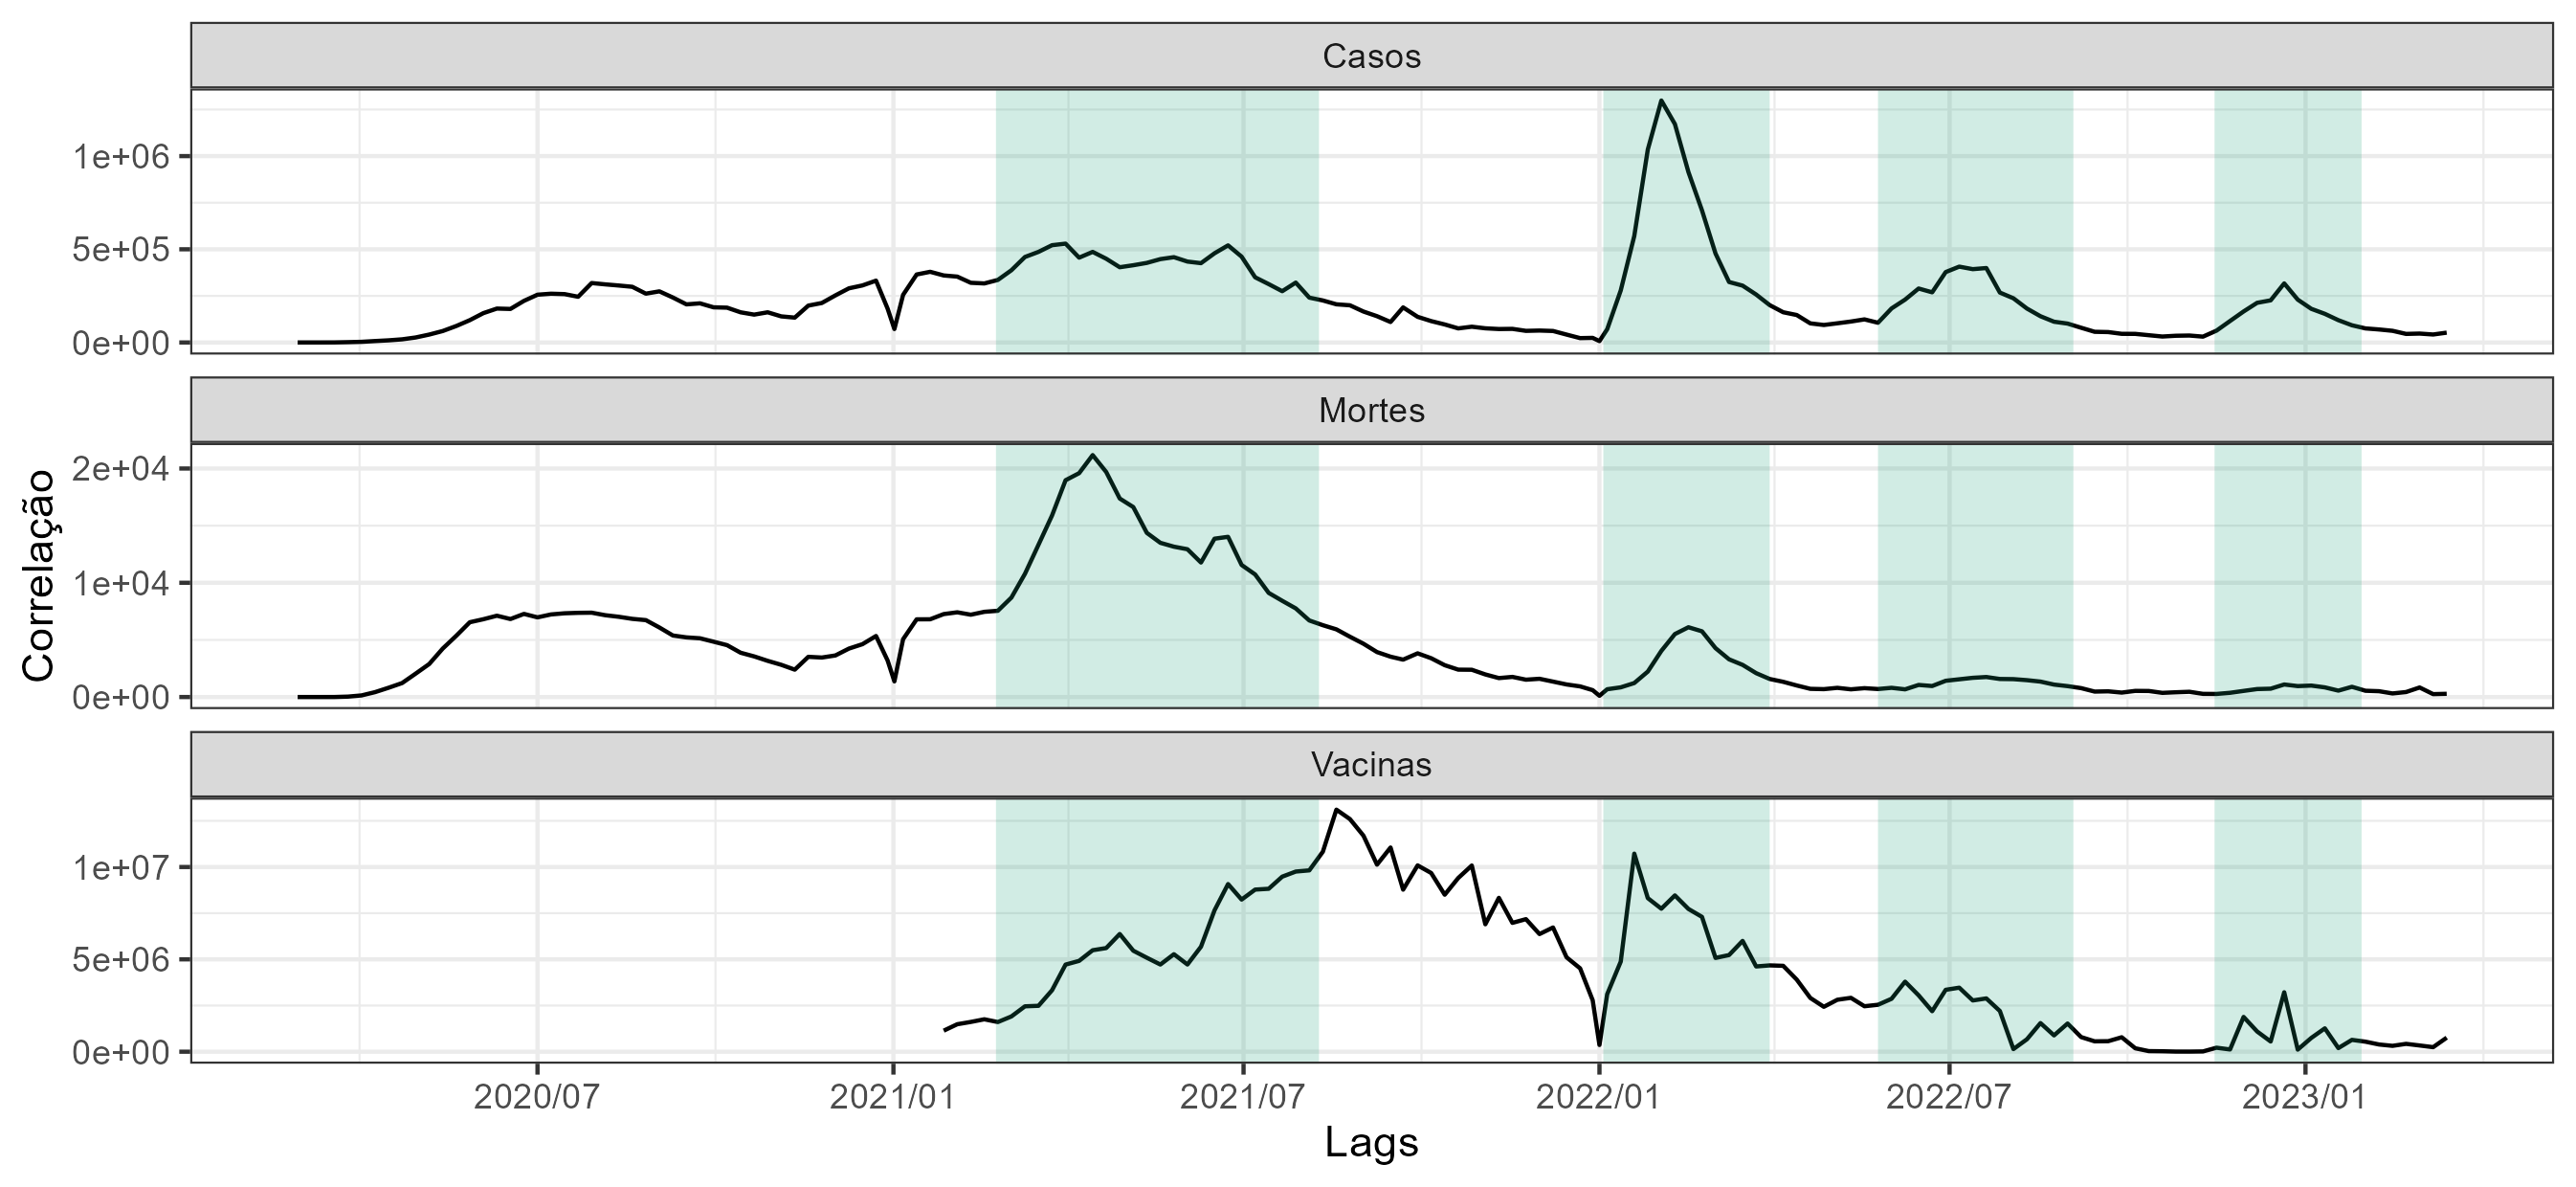
\includegraphics[width = 0.95\textwidth]{Figuras/stat_historic.png}
    \label{fig:histval}
\end{figure}

A figura \ref{fig:acfall} apresenta as autocorrelações (padrões, parciais, e cruzadas) das séries. As variáveis têm muitos \textit{lags} significativos em suas ACF's, e apenas os primeiros em suas PACF's. Alguns fatos interessantes: casos tem a maior auto dependência; vacinas tem maior relação com mortes do que com casos -- algo possivelmente relacionado com a ``preferência'' do governo, produtores, e ``tomadores de vacinas''; as outras variáveis não apresentam correlação negativa com vacinas.

\begin{figure}[H]
    \centering
    \caption{Correlação cruzada e parcial das séries}
    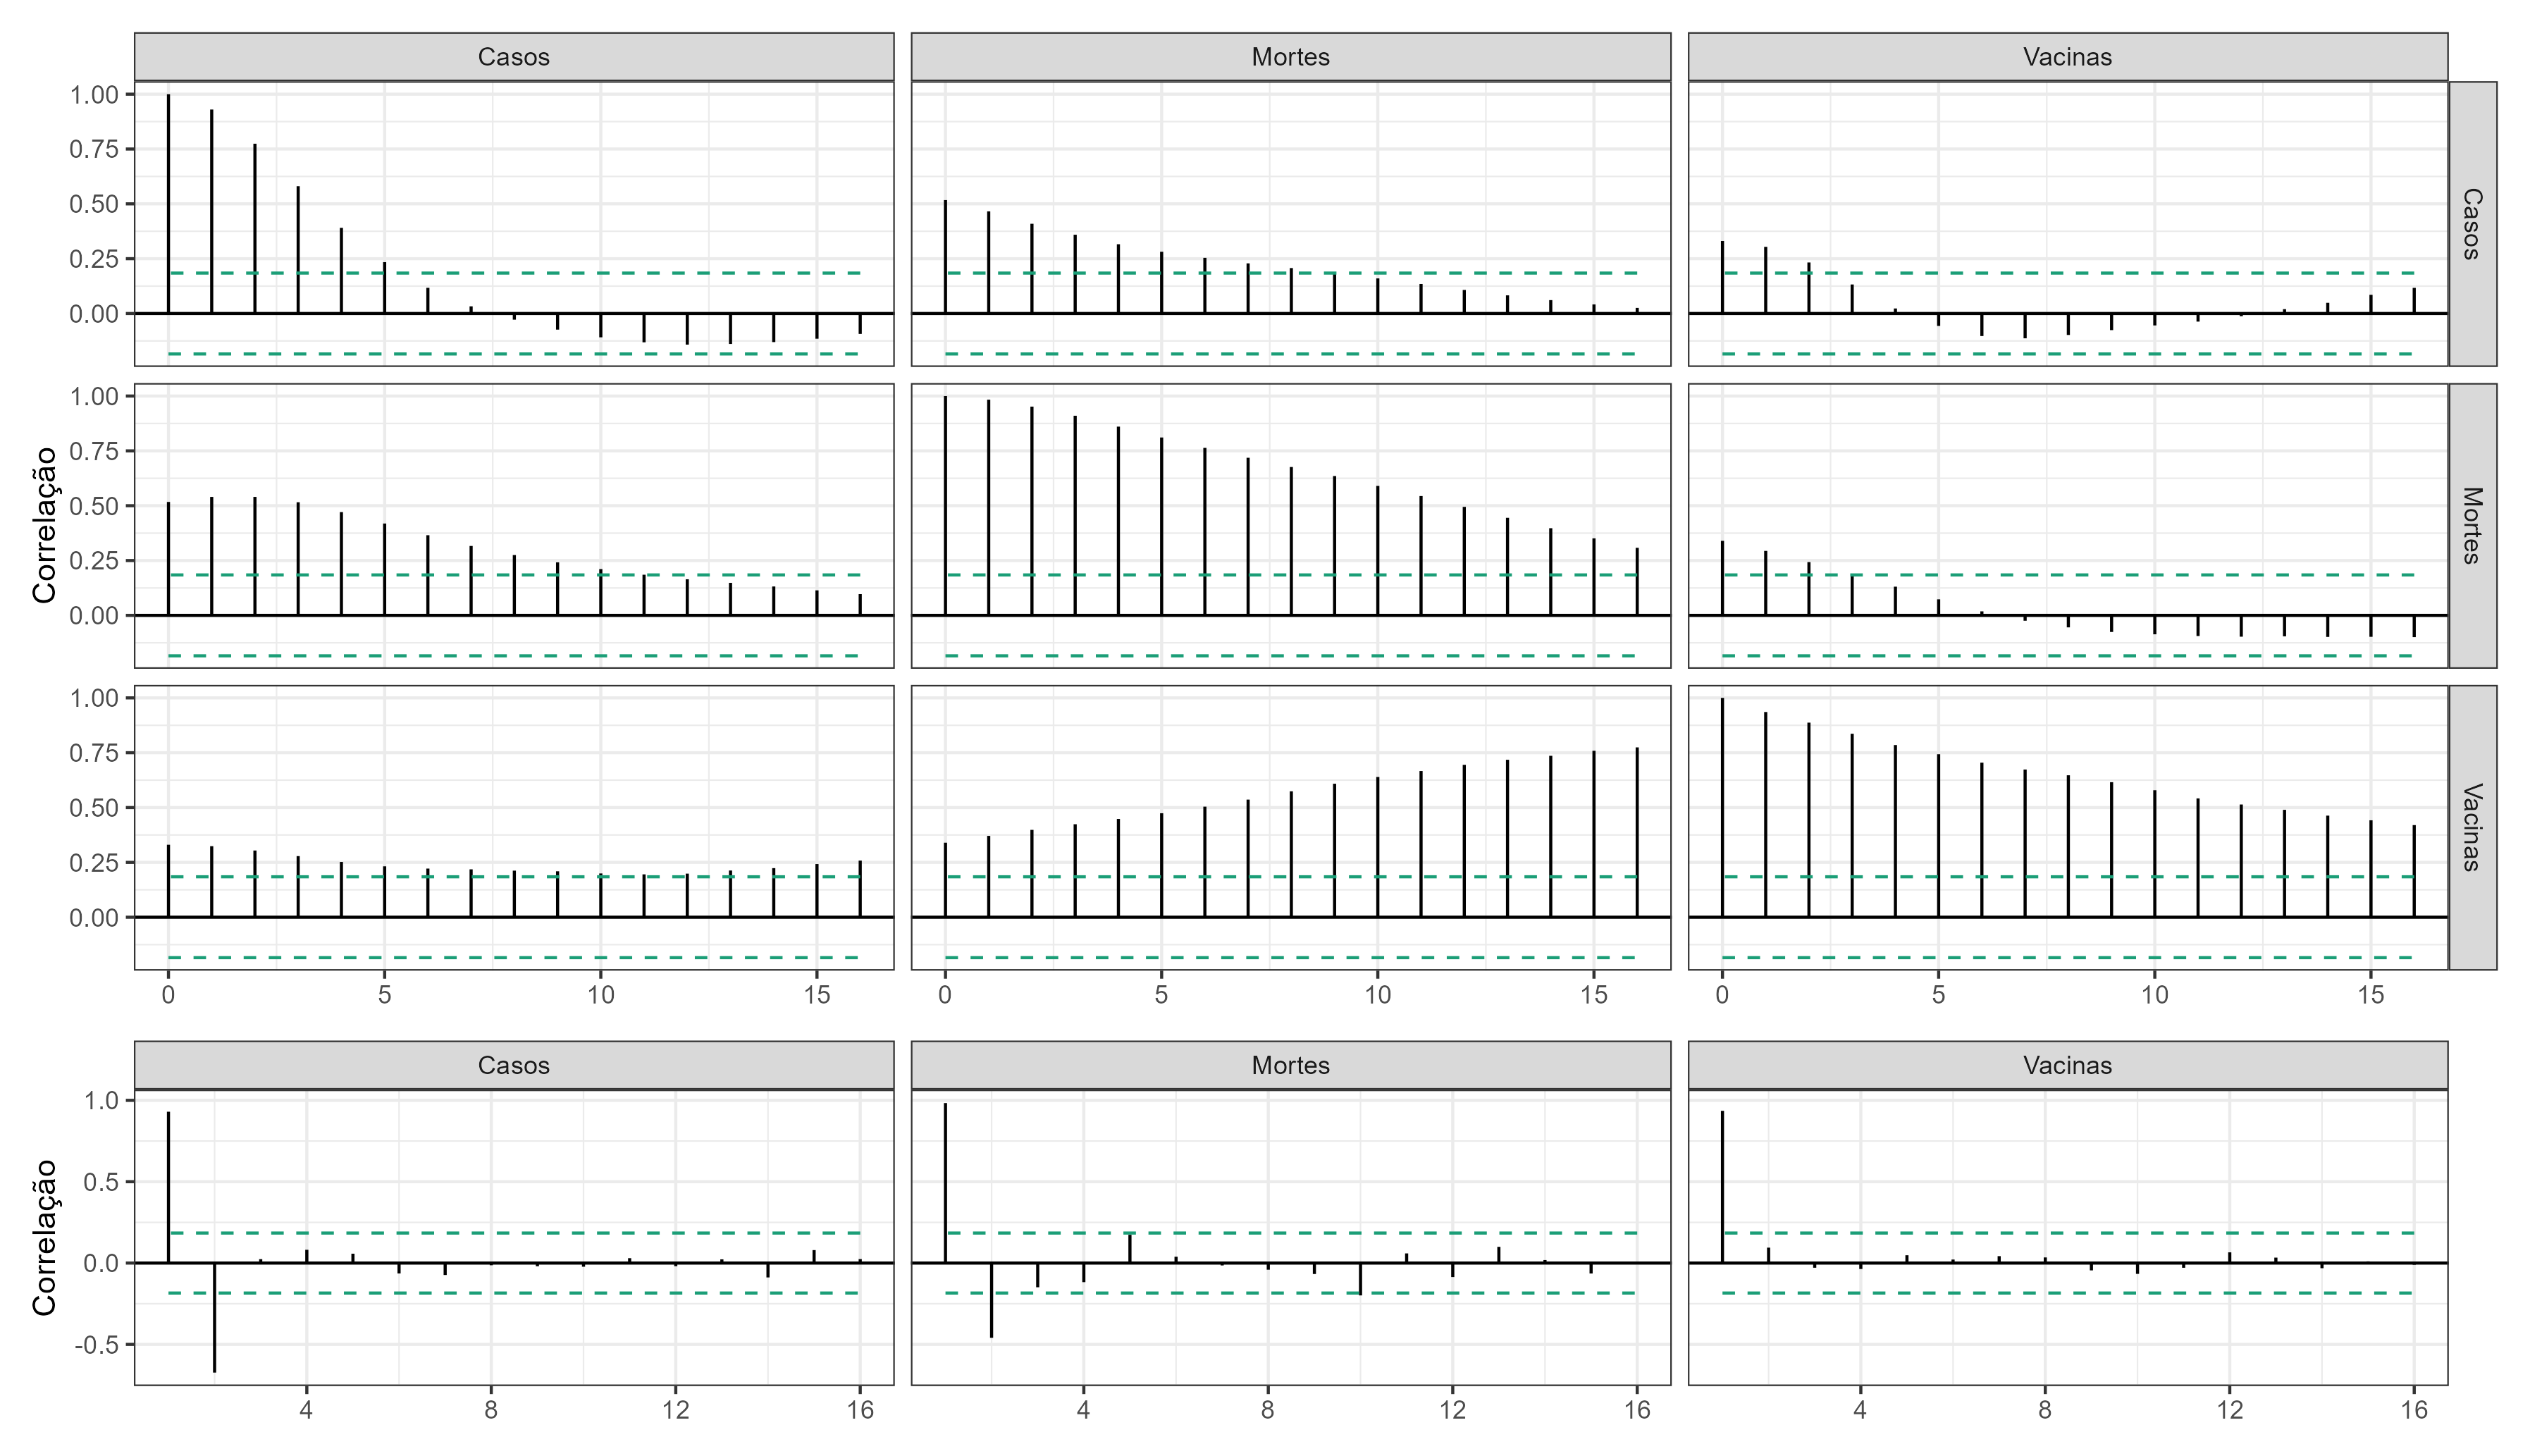
\includegraphics[width = 0.95\textwidth]{Figuras/stat_acf.png}
    \label{fig:acfall}
\end{figure}

Essa última constatação é contraintuitiva, e pode indicar como pode ser limitado medir o efeito direto da vacinação. Em oposição o efeito da vacina na relação das variáveis tem um resultado inicial interessante, exposto na figura \ref{fig:ccfad}. Uma análise das correlações cruzadas antes e depois da vacinação mostram uma maior relação entre \textit{lags} de casos e mortes no período pré vacina, possivelmente indicando um aumento na resistência contra a doença na população pós vacina. Essa diferença é ainda maior no cenário da política de vacinação mais avançada como, por exemplo, $10$ meses pós vacina.

\begin{figure}[H]
    \centering
    \caption{Correlação mortes-casos pré e pós vacinas}
    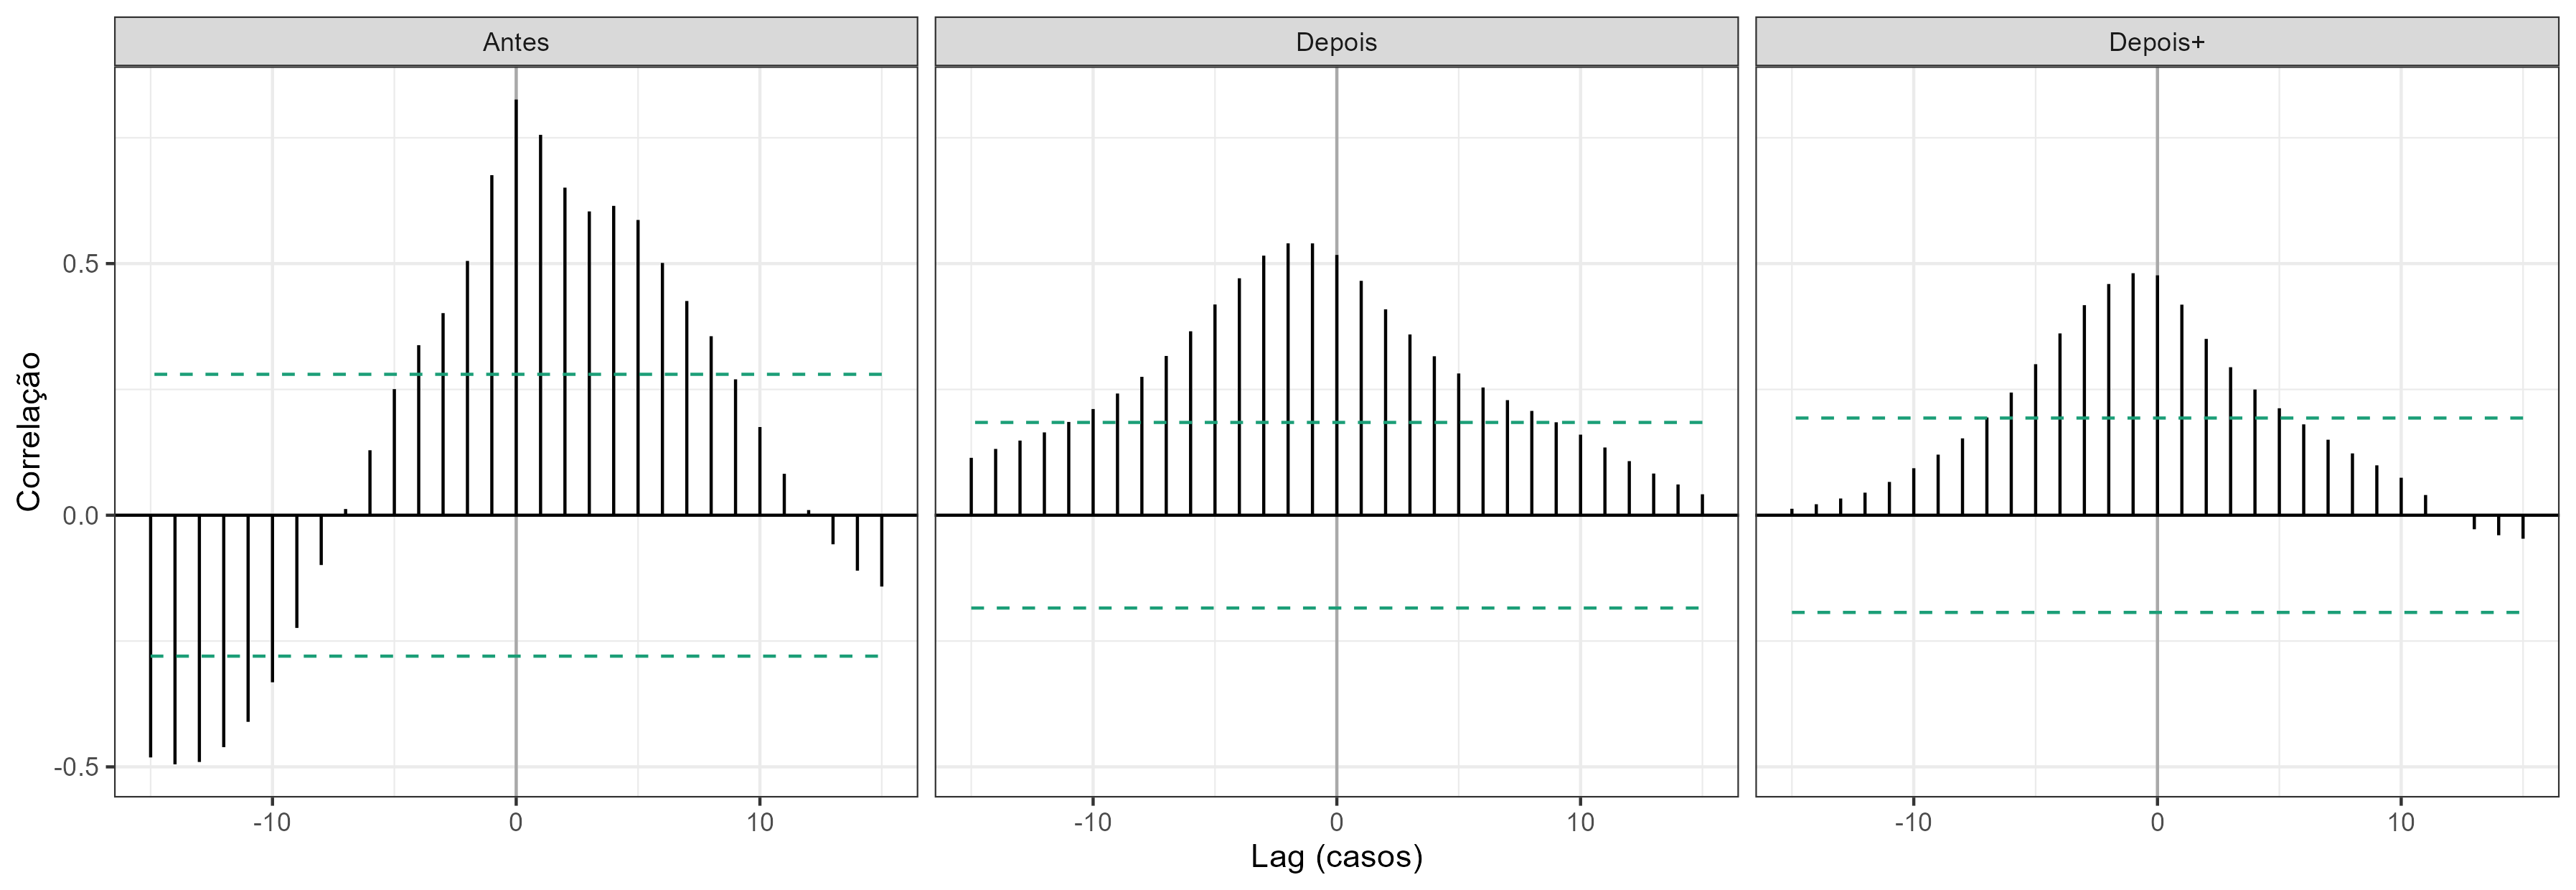
\includegraphics[width = 0.95\textwidth]{Figuras/stat_ba.png}
    \label{fig:ccfad}
\end{figure}

Por fim, no que tange a sazonalidade do COVID-19, a literatura é inconclusiva (\cite{Byun2021}). Alguns estudos atestam relação com a temperatura ao longo do ano (\cite{Wiemken2023}), porém, essa relação não pareceu estar tão significativa nos dados disponíveis, e gerou pouco efeito no modelo econométrico. Outras especificações de sazonalidade foram testadas, mas ao fim, nenhum tipo de correção pareceu necessária.



\let\clearpage\relax
\chapter{Modelo Econométrico}\label{sec:model}

Para realizar as três abordagens diferentes citadas na seção do modelo teórico, foram estimados os modelos \eqref{eq:var1} a \eqref{eq:var3}:

\begin{align}
&\begin{bmatrix}
I_t \\ D_t
\end{bmatrix}
= \alpha_0^{(1)} + \sum_{j=1}^{p^{(1)}}\pmb{\phi}_j^{(1)}
\begin{bmatrix}
I_{t-j} \\ D_{t-j}
\end{bmatrix}
+ \pmb{\alpha}^{(1)}_1onda_t + \pmb{\alpha}^{(1)}_2onda_t^2 + \pmb{\varepsilon}_{t}^{(1)}, \;\; t \in \{1, 2, ..., t_v\} \label{eq:var1}\\
&\text{Modelo (1) estimado na amostra } t \in \{t_v, t_v+1, ..., t_f\}\label{eq:var2}\\
&\begin{bmatrix}
I_t \\ V_t \\ D_t
\end{bmatrix}
= \alpha_0^{(3)} + \sum_{j=1}^{p^2}\pmb{\phi}_j^{(3)}
\begin{bmatrix}
I_{t-j} \\ V_{t-j} \\ D_{t-j}
\end{bmatrix}
+ \pmb{\alpha}^{(3)}_1onda_t + \pmb{\alpha}^{(3)}_2onda_t^2 + \pmb{\varepsilon}_{t}^{(3)}, \;\; t \in \{t_v, t_v+1, ..., t_f\}\label{eq:var3}\\
&\text{Modelo (1) estimado na amostra } t \in \{t_v+g, t_v+g+1, ..., t_f\}\label{eq:var4}\\
&\text{Modelo (3) estimado na amostra } t \in \{t_v+g, t_v+g+1, ..., t_f\}\label{eq:var5}
\end{align}

\noindent Onde $t_v$ é a data da primeira vacina e $t_f$ é a última data na base de dados. $V_t$ é o número de vacinas aplicadas no período $t$, $I_t$ é o número de casos registrados no período, e  $D_t$ é o número de mortes registrados no período. $onda_t$ é um vetor com um índice de tempo para cada onda (como definidas pela figura \ref{fig:histval}).

O modelo \eqref{eq:var1} é o modelo pré vacinação, \eqref{eq:var3} o modelo pós vacinação, e \eqref{eq:var2} um modelo ``intermediário''. Ele já apresenta a nova dinâmica entre casos e mortes pós vacinas, mas não leva em conta o efeito ``indireto" dessas variáveis com vacinas, por isso, a princípio, deve apresentar os efeitos positivos da vacinação, mas em menor intensidade do que o segundo \eqref{eq:var3}.

Os modelos \eqref{eq:var4} e \eqref{eq:var5} foram estimados considerando um ``\textit{gap}'' na amostra, para melhor separá-los do período pré vacinação. O \textit{gap} escolhido foi o menor que gerou uma diferença expressiva, $g = 10$ semanas.

A seleção do número de \textit{lags} $p$ para cada modelo, foi feita com base nos critérios de informação, e nos diagnósticos pós estimação. O modelo \eqref{eq:var1} teve $p = 1$, o resto $p = 2$. Todos os modelos foram estimados por MQO equação-a-equação. Os diagnósticos dos três modelos são similares, e os testes para o modelo \eqref{eq:var5} são apresentados no apêndice \ref{ap:diag}.

Em seguida os efeitos contemporâneos entre as variáveis foram modelados utilizando a decomposição de Cholesky, estimando os modelos estruturais. Foi feita a decomposição na ordem casos-vacinas-mortes, gerando a seguinte matrizes de relações contemporâneas:

\begin{equation}\label{eq:svar}
    \begin{bmatrix}
    \varphi_{II}^1 & 0 & 0 \\
    \varphi_{IV}^1 & \varphi_{VV}^1 & 0 \\
    \varphi_{ID}^1 & \varphi_{VD}^1 & \varphi_{DD}^1
    \end{bmatrix}
\end{equation}

Todo o trabalho computacional foi realizado utilizando o \textit{software} R com os pacotes \textit{vars}, \textit{svars}, e \textit{varutils}. O repositório de github com o código outras informações pode ser encontrado \href{https://github.com/ricardo-semiao/covid-svardiff}{neste link}.



\let\clearpage\relax
\chapter{Resultados e discussão}

A seção \ref{sec:res1} calcula as IRF's dos cinco modelos VAR, utilizando os modelos SVAR, mostrando como a inclusão de vacinas afeta as funções. A seção \ref{sec:res2} constrói contrafactuais da não existência de vacinas com vários métodos diferentes, utilizando os modelos VAR, obtendo estimativas do efeito total da política de vacinação. O apdêndice \ref{ap:single} mostra a análise não prioritária das IRF's do modelo (SVAR) \eqref{eq:var5}.

Antes de apresentar os resultados principais, vale a pena mostrar como correlação entre $\hat{\varepsilon}^i_{Casos}$ e $\hat{\varepsilon}^i_{Mortes}$\footnote{$\hat{\varepsilon}^i$ indica vetor de resíduos do modelo (i).} diminuiu após o início da vacinação. Nos três modelos VAR, respectivamente: $\mathbb{COR}(\hat{\varepsilon}^i_{Mortes}, \hat{\varepsilon}^i_{Casos}) = 0,91$, $0,46$, $0,48$, $0,30$, e $0,30$. Esse fato é uma evidência preliminar sobre como a vacina alterou a relação entre os choques das variáveis. A comparação completa das correlações e das matrizes contemporâneas dos SVAR'res pode ser vista no apêndice \ref{ap:corres}.


\section{Resposta de Mortes à Casos Pré e Pós Vacinação}\label{sec:res1}

O resultado principal deste trabalho é mostrar a diferença do impacto de um choque de casos pré e pós vacinação, algo que fica claro na figura \ref{fig:IRF BaA}, que mostra a função de resposta (em mortes) ao impulso (de $1000$ casos), para os cinco modelos\footnote{Intervalos de confiança não foram calculados por imprecisões nos pacotes disponíveis no R.}.

\begin{figure}[H]
    \centering
    \caption{IRF casos em mortes - modelos (1) a (5)}
    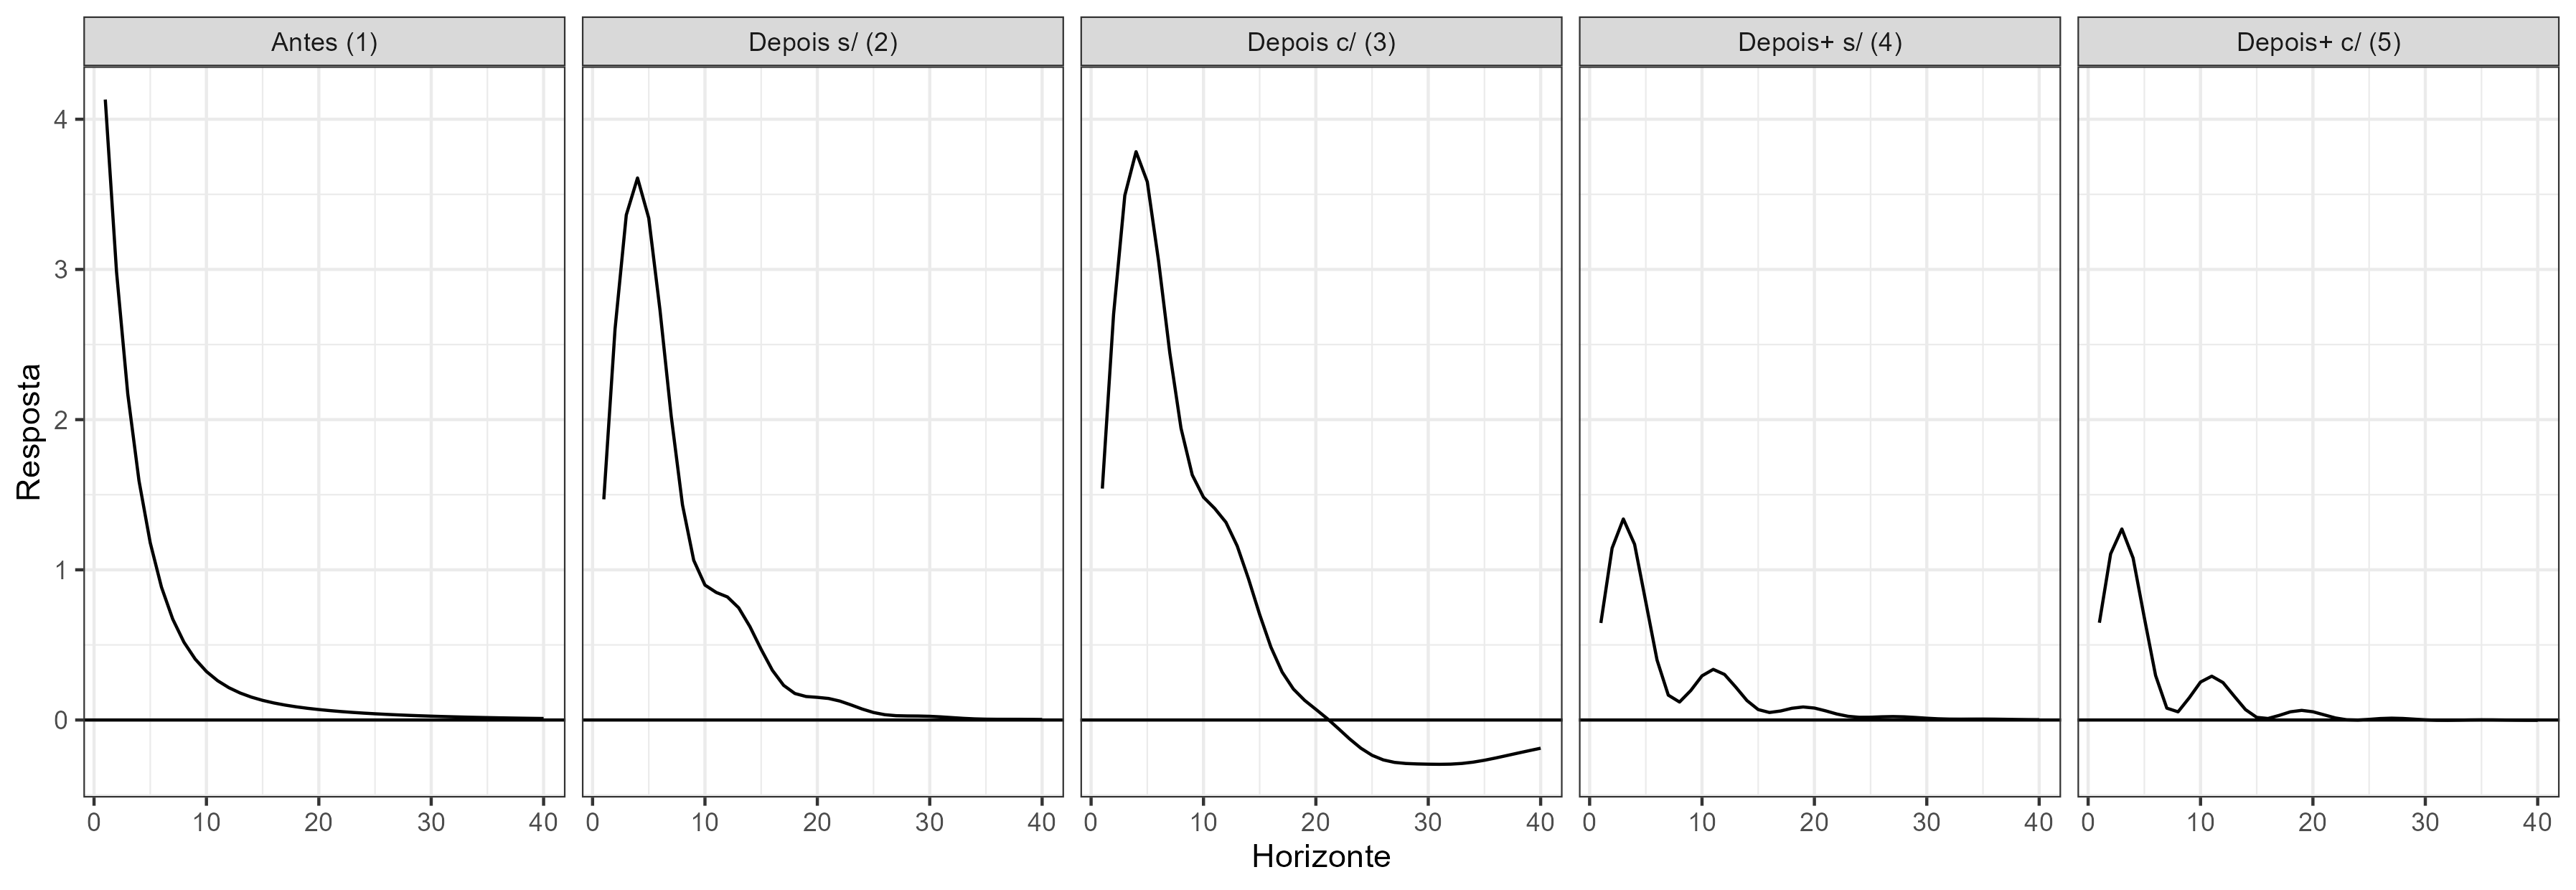
\includegraphics[width = 0.95\textwidth]{Figuras/res1_irfs.png}
    \label{fig:IRF BaA}
\end{figure}

Antes da vacinação, um choque de $1000$ casos gerava $4,13$ mortes na primeira semana. Após a vacina, os modelos sem \textit{gap} indicam um primeiro choque em torno de $1,5$, e os com, um choque próximo de $0,64$.

Só o pico não passa toda a mudança de dinâmica, a vacinação pode afetar também a trajetória das funções: existem os efeitos sobre a confiança e distanciamento; o tempo de cama antes do falecimento pode aumentar; além de possivelmente afetar a própria taxa de mortalidade.

Por esse motivo, vale também analisar as mudanças nas somas dos valores das funções (tabela \ref{tb:irfsoma}). A soma da resposta à $1000$ casos é de $16,91$ mortes, reduzindo para $7,99$ no modelo intermediário, e $6,67$ no último modelo (ambos com \textit{gap}), representando uma diminuição na resposta de $10,24$ mortes (ou 40\%).

Os modelos sem \textit{gap} mostram um aumento grande nas respostas, totalizando, contraintuitivamente, um maior número de mortes. Esse resultado deve estar relacionado à má separação dos momentos pré e pós desses modelos, indicando a superioridade dos modelos com \textit{gap}.

\begin{table}[H]
\centering
\caption{Variações na Soma das IRF's}
\label{tb:irfsoma}
\begin{tabular}{cccc}
\\[-1.8ex]\hline 
\hline \\[-1.8ex] 
Modelo & Estimativa & (1) - (i) & \%\\\hline\\[-1.8ex]
\multicolumn{1}{c|}{\eqref{eq:var1}}    & 16,91  & 0     & 100\%\\ 
\multicolumn{1}{c|}{\eqref{eq:var2}}    & 27,81  & $<0$    & $<0$   \\ 
\multicolumn{1}{c|}{\eqref{eq:var3}}    & 26,91  & $<0$    & $<0$   \\
\multicolumn{1}{c|}{\eqref{eq:var4}}    & 7,99   & 8,92  & 53\% \\
\multicolumn{1}{c|}{\eqref{eq:var5}}    & 6,67   & 10,24 & 60\% \\
\\[-1.8ex]\hline 
\hline \\[-1.8ex] 
\end{tabular}
\end{table}

É importante lembrar que as IRF's analisadas são aproximações lineares das respostas durante o período analisado, sem permitir variações nessas funções com base nos níveis das outras variáveis, algo que o modelo SIRDV assumia ser importante. Se, por exemplo, a resposta à vacinas cai muito conforme o número de imunizados sobe, essa metodologia deve apresentar um resultado muito superestimado.

Por último, note que estamos interpretando a IRF sem vacina como um contrafactual da ``IRF no período pós vacinas, mas no mundo onde a vacinação não ocorreu''\footnote{A princípio essa interpretação faz sentido, como discutido no final da seção \ref{sec:teorico2}}. Com isso em mente, podemos extrapolar os resultados dessa seção, e multiplicar a IRF sem vacinas pelo total de casos\footnote{Dividido por mil, uma vez que essa era o tamanho do choque.}. Os resultados desse método são apresentados no fim da seção seguinte.


\section{Análise de Contrafactual}\label{sec:res2}

Para ter uma medida do efeito total da política de vacinação, é possível construir um contrafactual onde nunca houve a vacinação, e comparar com os casos e mortes observados. Para isso, foram elencados alguns métodos diferentes: (i) utilizar o modelo \eqref{eq:var1} para ``prever'' o período pós vacinas; (ii) utilizar o modelo \eqref{eq:var5}\footnote{Os resultados utilizando o modelo \eqref{eq:var3} são similares} para ``prever'' a série de casos e mortes (a partir do ponto pré vacinas), mas zerando o efeito das vacinas; (iii) usar o contrafatual de casos como ``choque total'' e multiplicar pela IRF sem vacinas da seção anterior. (i*), (ii*), e (iii*) envolvem as mesmas duas abordagens anteriores, mas em vez de calcular a variável de casos com o modelo, utilizar a variável de casos observada para calcular um contrafactual apenas para mortes.

Alguns comentários sobre cada abordagem:

\begin{itemize}
    \item Os contrafactuais são diferentes:
    \begin{itemize}
    \item (i*) a (iii*) estimam ``qual seria o número de mortes no 'mundo' sem vacinas, mas onde os casos se mantiveram iguais?'';
    \item (i) a (iii) estimam ``qual seria o número de mortes no mundo sem vacinas, dado que a falta de vacinas também afeta o número de casos?'';
\end{itemize}
    \item (i) a (iii) são mais ``completos'' mas dependem da problemática interpretação da variável de casos. (i*) a (iii*) são mais ``conservadores'', mas mais precisos.
    \item (i*) a (iii*) também são mais conservadores por já carregar a mudança na relação entre as variáveis em seus coeficientes;
    \item (i) e (i*) foram estimados com metade das observações de (ii) e (ii*). Adicionalmente, (i) não tem muita informação para ``prever'' trajetórias, e deve ser um método ainda mais errático;
    \item (iii) e (iii*) são métodos menos tradicionais, extrapolando os choques individuais ao nível agregado, com alto potencial de superestimação.
    \item Por fim, todos os modelos utilizaram as tendências determinísticas. Embora no contrafactual as ondas poderiam não ter ocorrido, os métodos não tem poder para determinar isso\footnote{Adicionalmente, as ondas estão relacionadas ao surgimento de variantes, algo exógeno ao contrafactual.}.
\end{itemize}

Em suma, estamos mais interessados no método (ii*) como o mais concervador, (ii) como uma opção menos conservadora, e (iii*) como uma abordagem adicional, potencialmente superestimada.

Os resultados dos métodos (i) e (ii) podem ser vistos na figura \ref{fig:counter1}. A figura apresenta o intervalo de confiança de $80$\%. Como esperado, o método (i) é bastante errático, mas o outro segue as séries realizadas com muito mais precisão.

\begin{figure}[H]
    \centering
    \caption{Contrafactuais (i) e (ii)}
    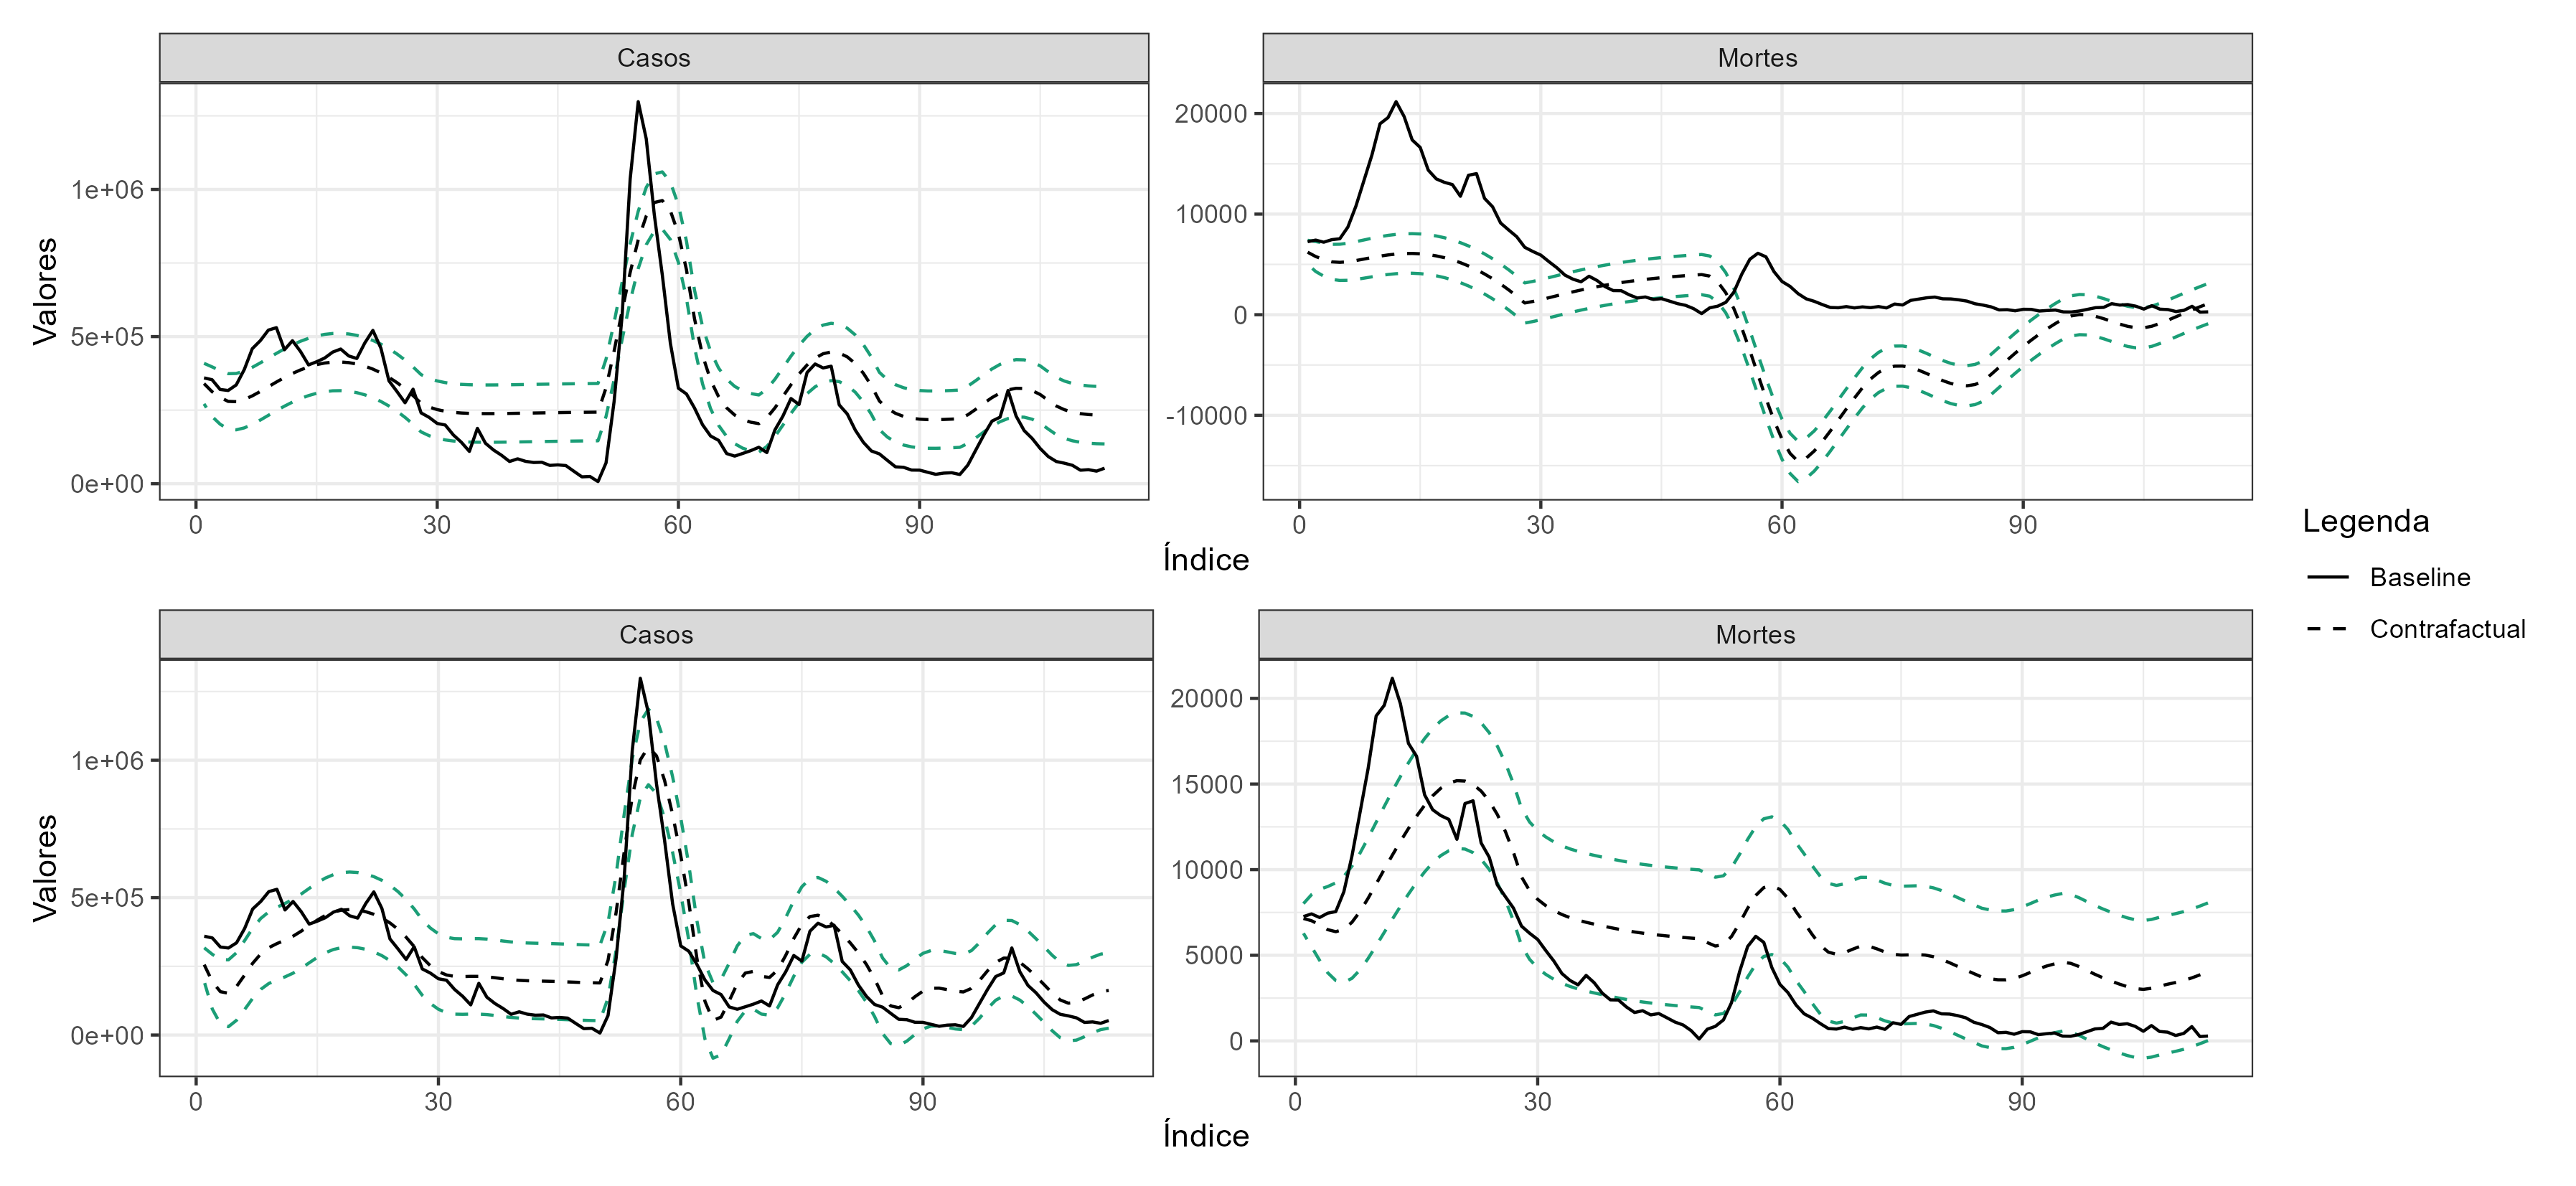
\includegraphics[width = 0.95\textwidth]{Figuras/res2_cf1-2.png}
    \label{fig:counter1}
\end{figure}

Os resultados dos métodos (i*) e (ii*) podem ser vistos na figura \ref{fig:counter2}. Os contrafactuais são realmente pouco disruptivos.

\begin{figure}[H]
    \centering
    \caption{Contrafactuais (i*) e (ii*)}
    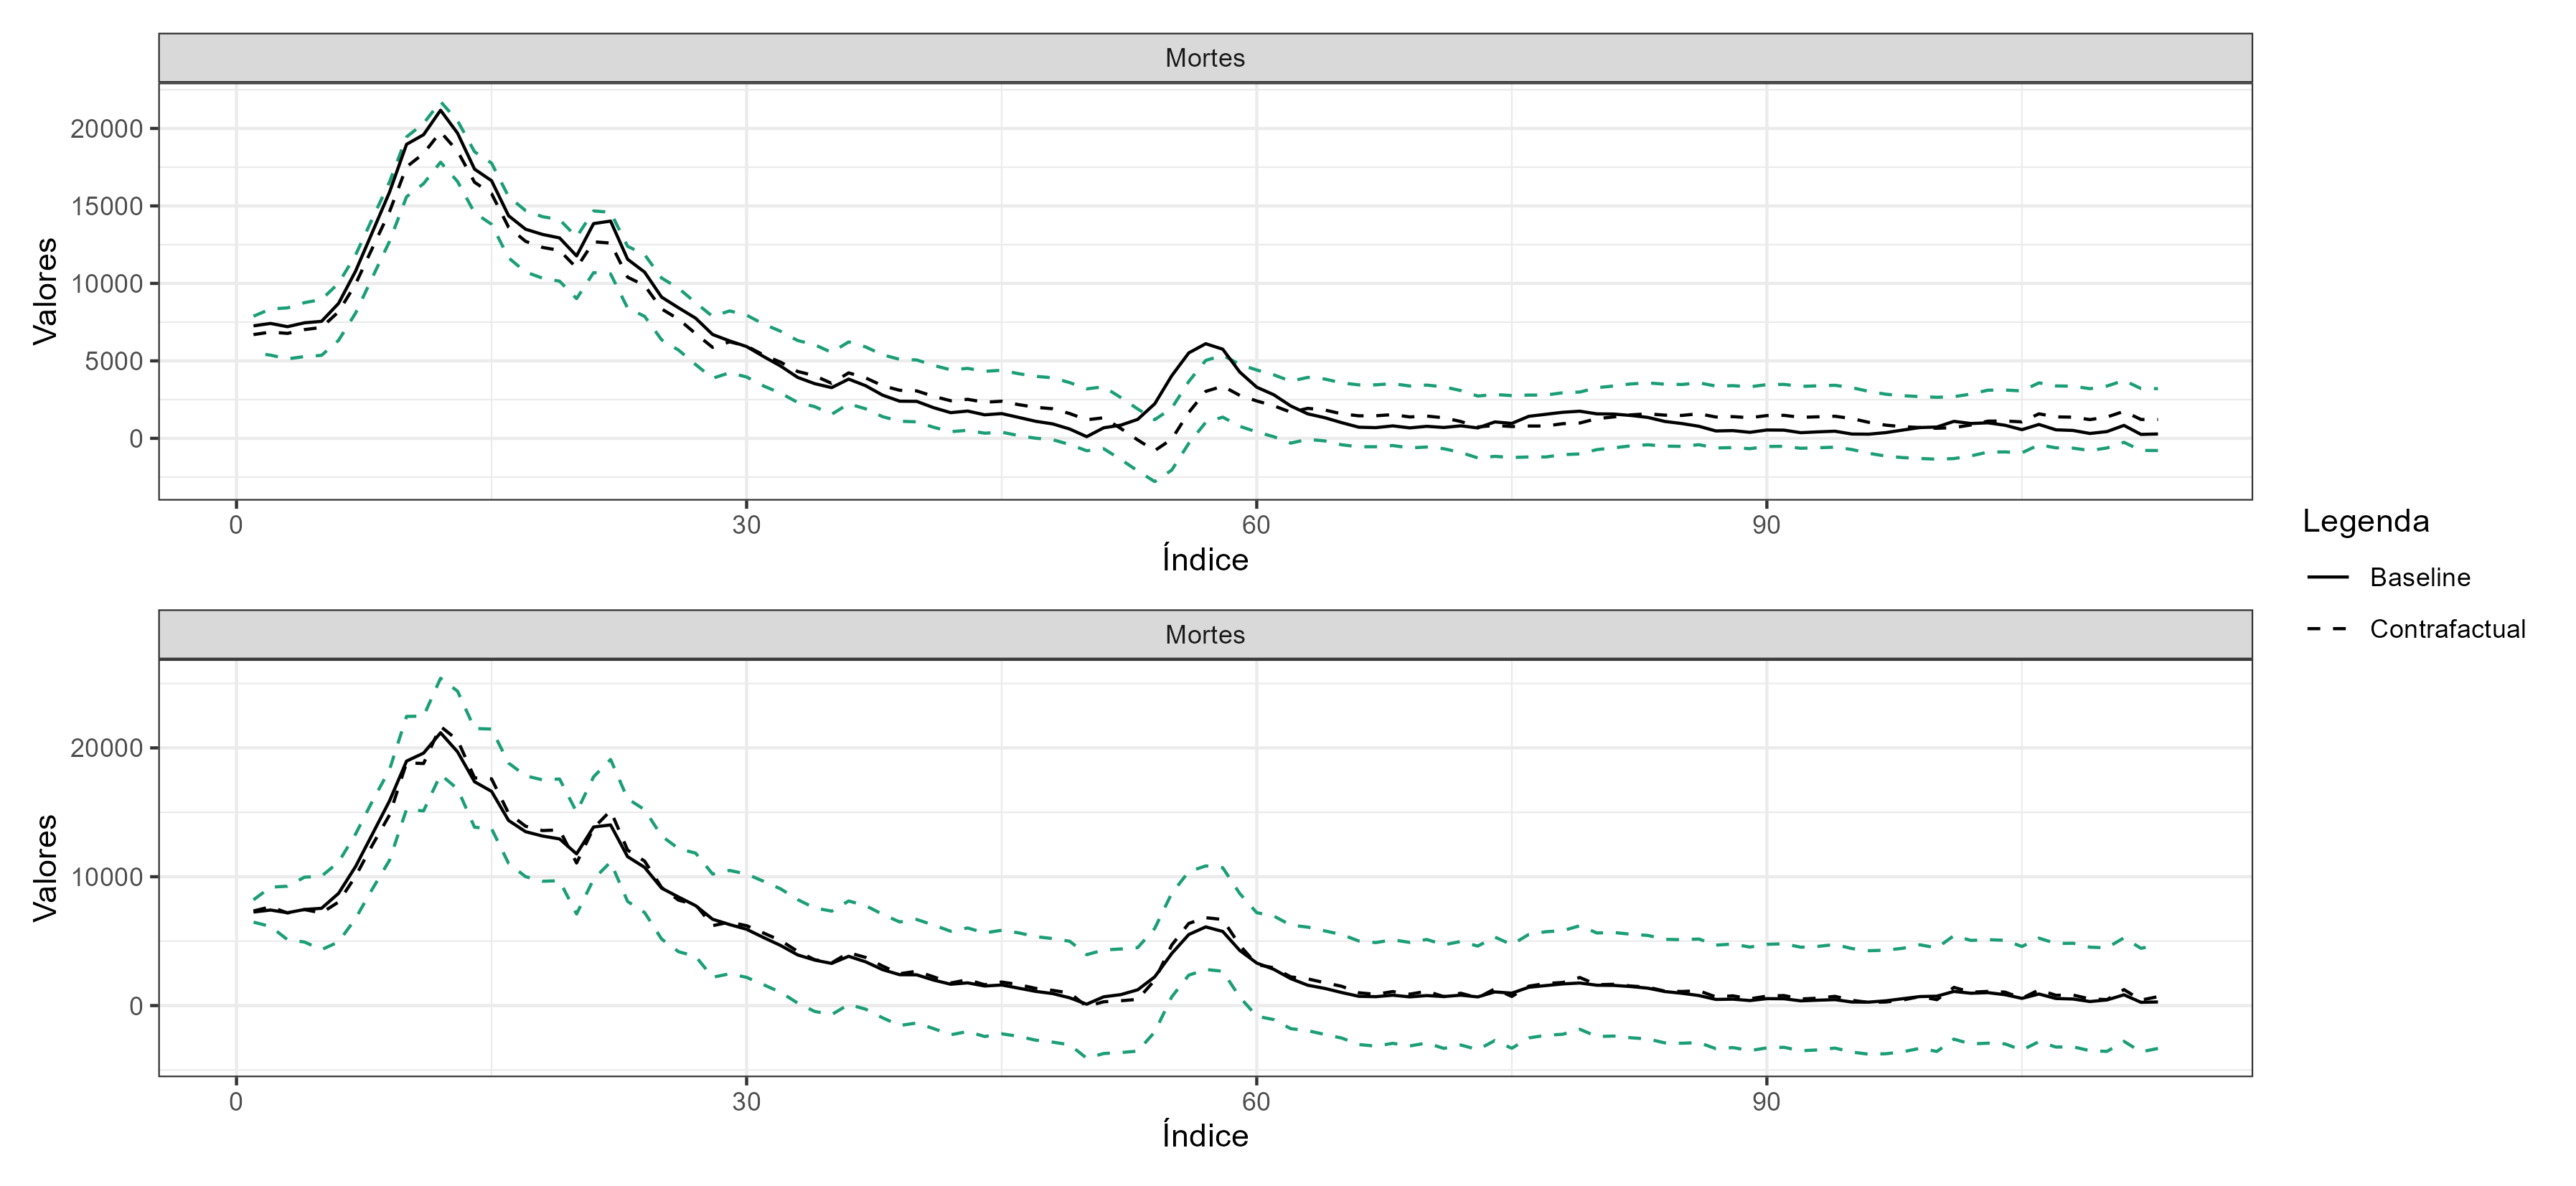
\includegraphics[width = 0.95\textwidth]{Figuras/res2_cf4-5.png}
    \label{fig:counter2}
\end{figure}

A construção do contrafactual multiplicando a série de casos pela IRF sem vacinas é limitada. A IRF é uma média das respostas, e na realidade, mortes não respondem sempre da mesma forma. na figura \ref{fig:counter3}, realmente vemos o descasamento das séries. Isso motiva a criação de outro \textit{baseline}, mais comparável, multiplicando a série de casos pela IRF com vacinas (modelo \eqref{eq:var5}). Embora essa comparação não seja exatamente na mesma ordem das outras abordagens, efetivamente transformamos a disparidade das IRF's em uma medida de quantidade total\footnote{Os segmentos em verde são a diferença contrafactual $-$ \textit{baseline}}.

\begin{figure}[H]
   \centering
   \caption{Contrafactuais (iii) e (iii*)}
   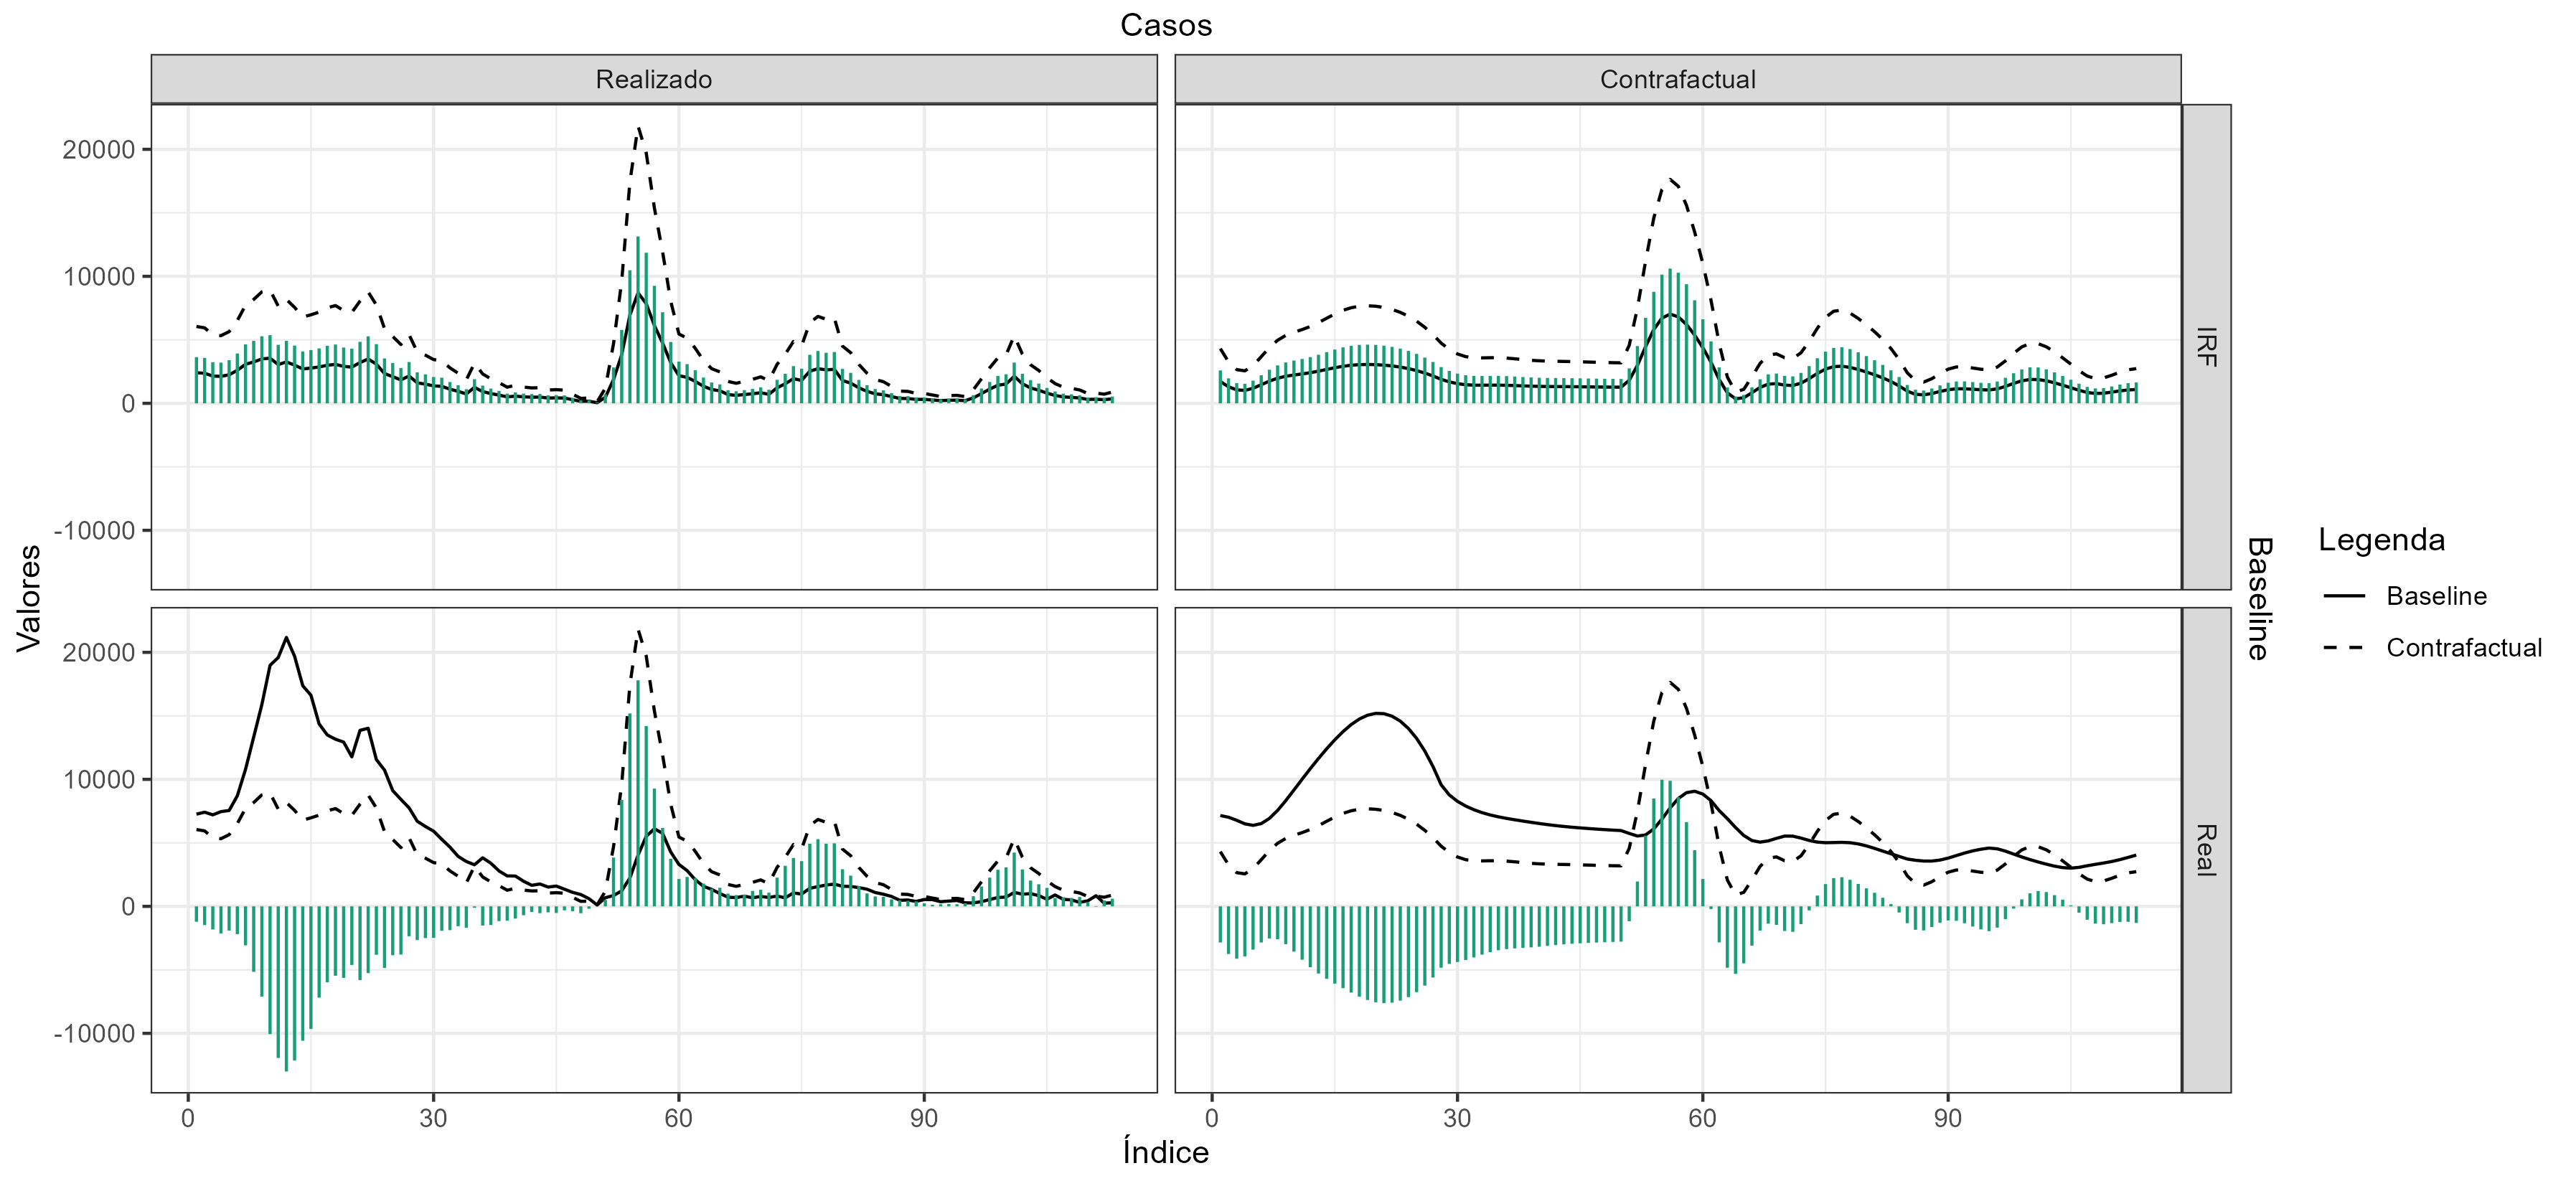
\includegraphics[width = 0.95\textwidth]{Figuras/res2_cf3-6.png}
   \label{fig:counter3}
\end{figure}

A tabela \ref{tb:counter} apresenta os modelos (ii), (ii*), (iii), e (iii*). Vemos que o contrafactual de casos realmente é limitado, apresentando uma banda de $30$ milhões de casos, enfraquecendo a confiança nos métodos que o utilizam. A abordagem (ii*) apresenta um resultado bastante conservador, $16$ mil ``vidas salvas''\footnote{Um valor substancialmente menor do que aquele calculado por \cite{Ferreira2021}}. Os outros métodos, por sua vez, realmente apresentaram números mais expressivos, tanto pelo uso do contrafactual de casos, quanto pela aproximação feita na IRF.

\begin{table}[H] \centering 
\renewcommand{\arraystretch}{1.2}
  \caption{Análise de Contrafactual}\label{tb:counter}
\begin{tabular}{@{\extracolsep{5pt}} llccc} 
\\[-1.8ex]\hline 
\hline \\[-1.8ex] 
Método & Série & Diferença & Int. inferior & Int. superior \\ 
\hline \\[-1.8ex] 
\multirow{2}{*}{(ii)} & Casos  & 4.873.072 & -10.424.667   & 20.170.811 \\ 
                      & Mortes & 279.473     & -159.341      & 718.288 \\ 
(ii*)                 & Mortes & 16.024    & -422.701      & 454.750  \\ 
(iii)                 & Mortes & 289.089    & -       & - \\
(iii*)                & Mortes & 338.402    & -        & - \\
\\[-1.8ex]\hline
\hline \\[-1.8ex]
\end{tabular} 
\end{table} 



\let\clearpage\relax
\chapter{Conclusão}

Nesta tese, foram desenvolvidas diferentes abordagens para medir medido efeito das vacinas no número de casos mortes que o Brasil apresentou durante a pandemia do COVID-19.

O uso de um modelo SVAR se mostrou atrativo. O modelo teórico SIRDV e os dados explicitaram a natureza de dinâmica temporal entre as variáveis; a teoria epidemiológica motivou a identificação estrutural; e foi possível obter diversas ordens de resultados.

A abordagem mais robusta comparou as IRF's de SVAR'es estimados antes e depois do início da vacinação, controlando possíveis falhas na especificação do modelo ao analisar como a vacina o altera. Essa abordagem mostrou a mudança na soma da resposta em mortes, dado um choque de $1000$ casos, é de $10,24$ em termos absolutos, e $60$\% em termos proporcionais, indicando o alto nível de eficiência da política de vacinação.

A outra abordagem foi a criação de um contrafactual para estimar o efeito agregado da vacinação. Foi identificado um \textit{lower} e um \textit{upper bound} de, respectivamente $16$ mil e $279$ mil vidas salvas até mar/2023. O valor real deve se encontrar longe dos \textit{bounds} uma vez que os valores apresentam indícios de sub/superestimação (respectivamente). Também foi criado um contrafactual com base na redução da IRF comentada anteriormente, e este é mais consistente com uma redução da ordem do supracitado \textit{upper bound}.

Esta tese apresentou mais uma metodologia para atestar a eficiência da vacinação, servindo como mais um insumo para a busca de um consenso na literatura e fim da desinformação, além de ser mais uma ferramenta para os \textit{policymakers} definirem o gasto e urgência ótima para as políticas de vacinação.

O potencial da metodologia não foi explorado até o fim, existe espaço para a busca de novas técnicas de identificação, busca de dados de melhor qualidade, inclusão do distanciamento social e não linearidade nos modelos. Com isso, seria possível aprimorar as estimativas obtidas, e possibilitar analisar as IRF's de vacinas em mortes e casos, gerando um resultado de efeito marginal muito útil. Similarmente, existe muito espaço para aplicações dessa metodologia em outros contextos para evidenciar seu bom funcionamento.



% ELEMENTOS PÓS TEXTUAIS ----------------------------------------
\postextual

% Referências bibliográficas:
\newpage
\printbibliography

% Apêndices:
\newpage
\begin{apendicesenv}

\setlength{\afterchapskip}{0.25\baselineskip}
\setlength{\beforechapskip}{0\baselineskip}

\chapter{Diagnósticos do VAR}\label{ap:diag}
Antes de sua inclusão no VAR \eqref{eq:var5}, foi realizado um teste de raiz unitária sobre as séries, apresentado na tabela \ref{tb:testadf}. Podemos ver que apenas a variável de casos é estacionária. Uma boa especificação do modelo pareceu lidar bem com essa limitação.

\begin{table}[H] \centering 
  \caption{Teste Dickey-Fuller Aumentado} 
  \label{tb:testadf} 
\begin{tabular}{@{\extracolsep{5pt}} cccc} 
\\[-1.8ex]\hline 
\hline \\[-1.8ex] 
Variável & Estatística & Lag & P-valor \\ 
\hline \\[-1.8ex] 
Casos & -3.61 & 5 & 0.03 \\ 
Vacinas & -2.97 & 4 & 0.17 \\ 
Mortes & -2.71 & 5 & 0.28 \\ 
\hline \\[-1.8ex] 
\end{tabular} 
\end{table} 

A figura \ref{fig:varfit} apresenta o fit e os resíduos do modelo. A distribuição dos resíduos parece relativamente ter uma volatilidade similar ao longo da reta de valores fitados, e de fato, o teste ARCH-LM não indicou a presença de erros ARCH no modelo -- estatística do teste de $206,61$, com $180$ graus de liberdade, gerando um p-valor $< 0,0848$. O R quadrado de cada equação é: Casos $0,960$, Vacinas $0,918$, Mortes $0,988$

\begin{figure}[H]
    \centering
    \caption{Fit e resíduos}
    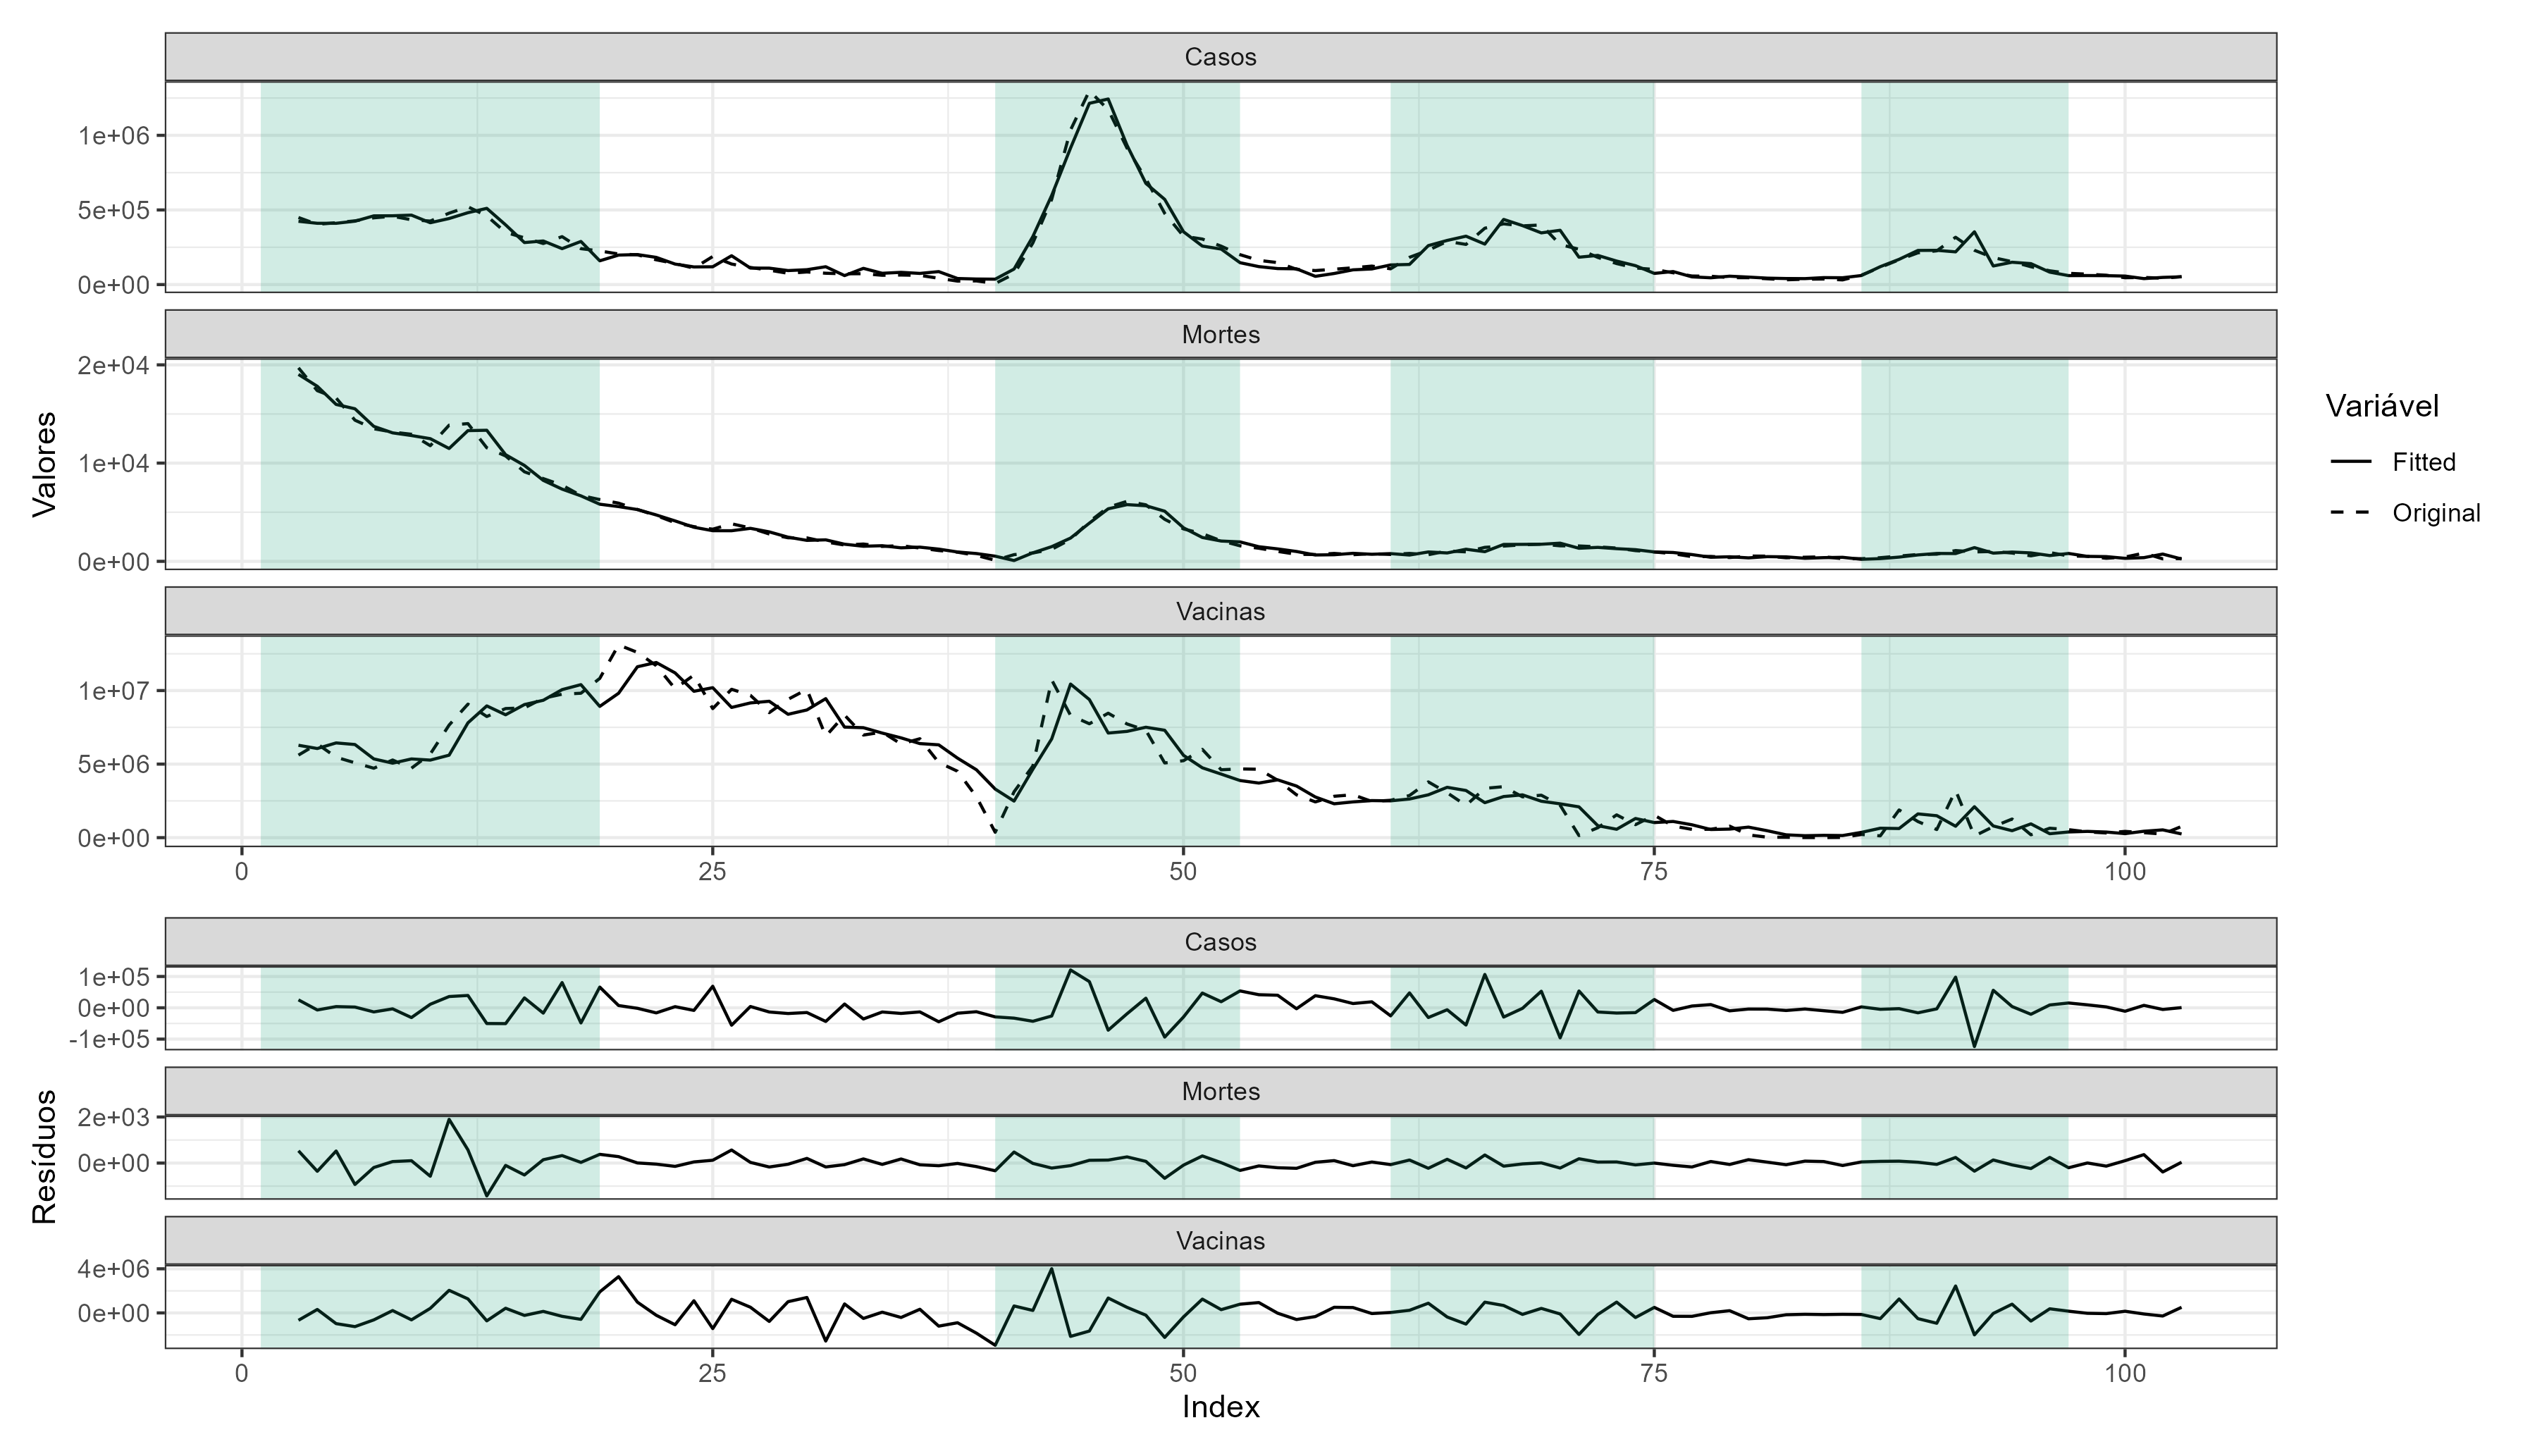
\includegraphics[width = 0.95\textwidth]{Figuras/diag_fit-res.png}
    \label{fig:varfit}
\end{figure}

Podemos ver mais detalhes dos resíduos na figura \ref{fig:varresdist}, que mostra uma variância dos resíduos não tão dependente dos valores do modelo, mas uma distribuição não exatamente normal. Realmente, o teste Jarque-Bera multivariado indica erros não normais -- estatística do teste de $42,113$, com $6$ graus de liberdade, gerando um p-valor de $1,747e-07$. Dito isso, esse resultado não compromete nenhuma hipótese deste trabalho.

\begin{figure}[H]
    \centering
    \caption{Dispersão e distribuição dos resíduos}
    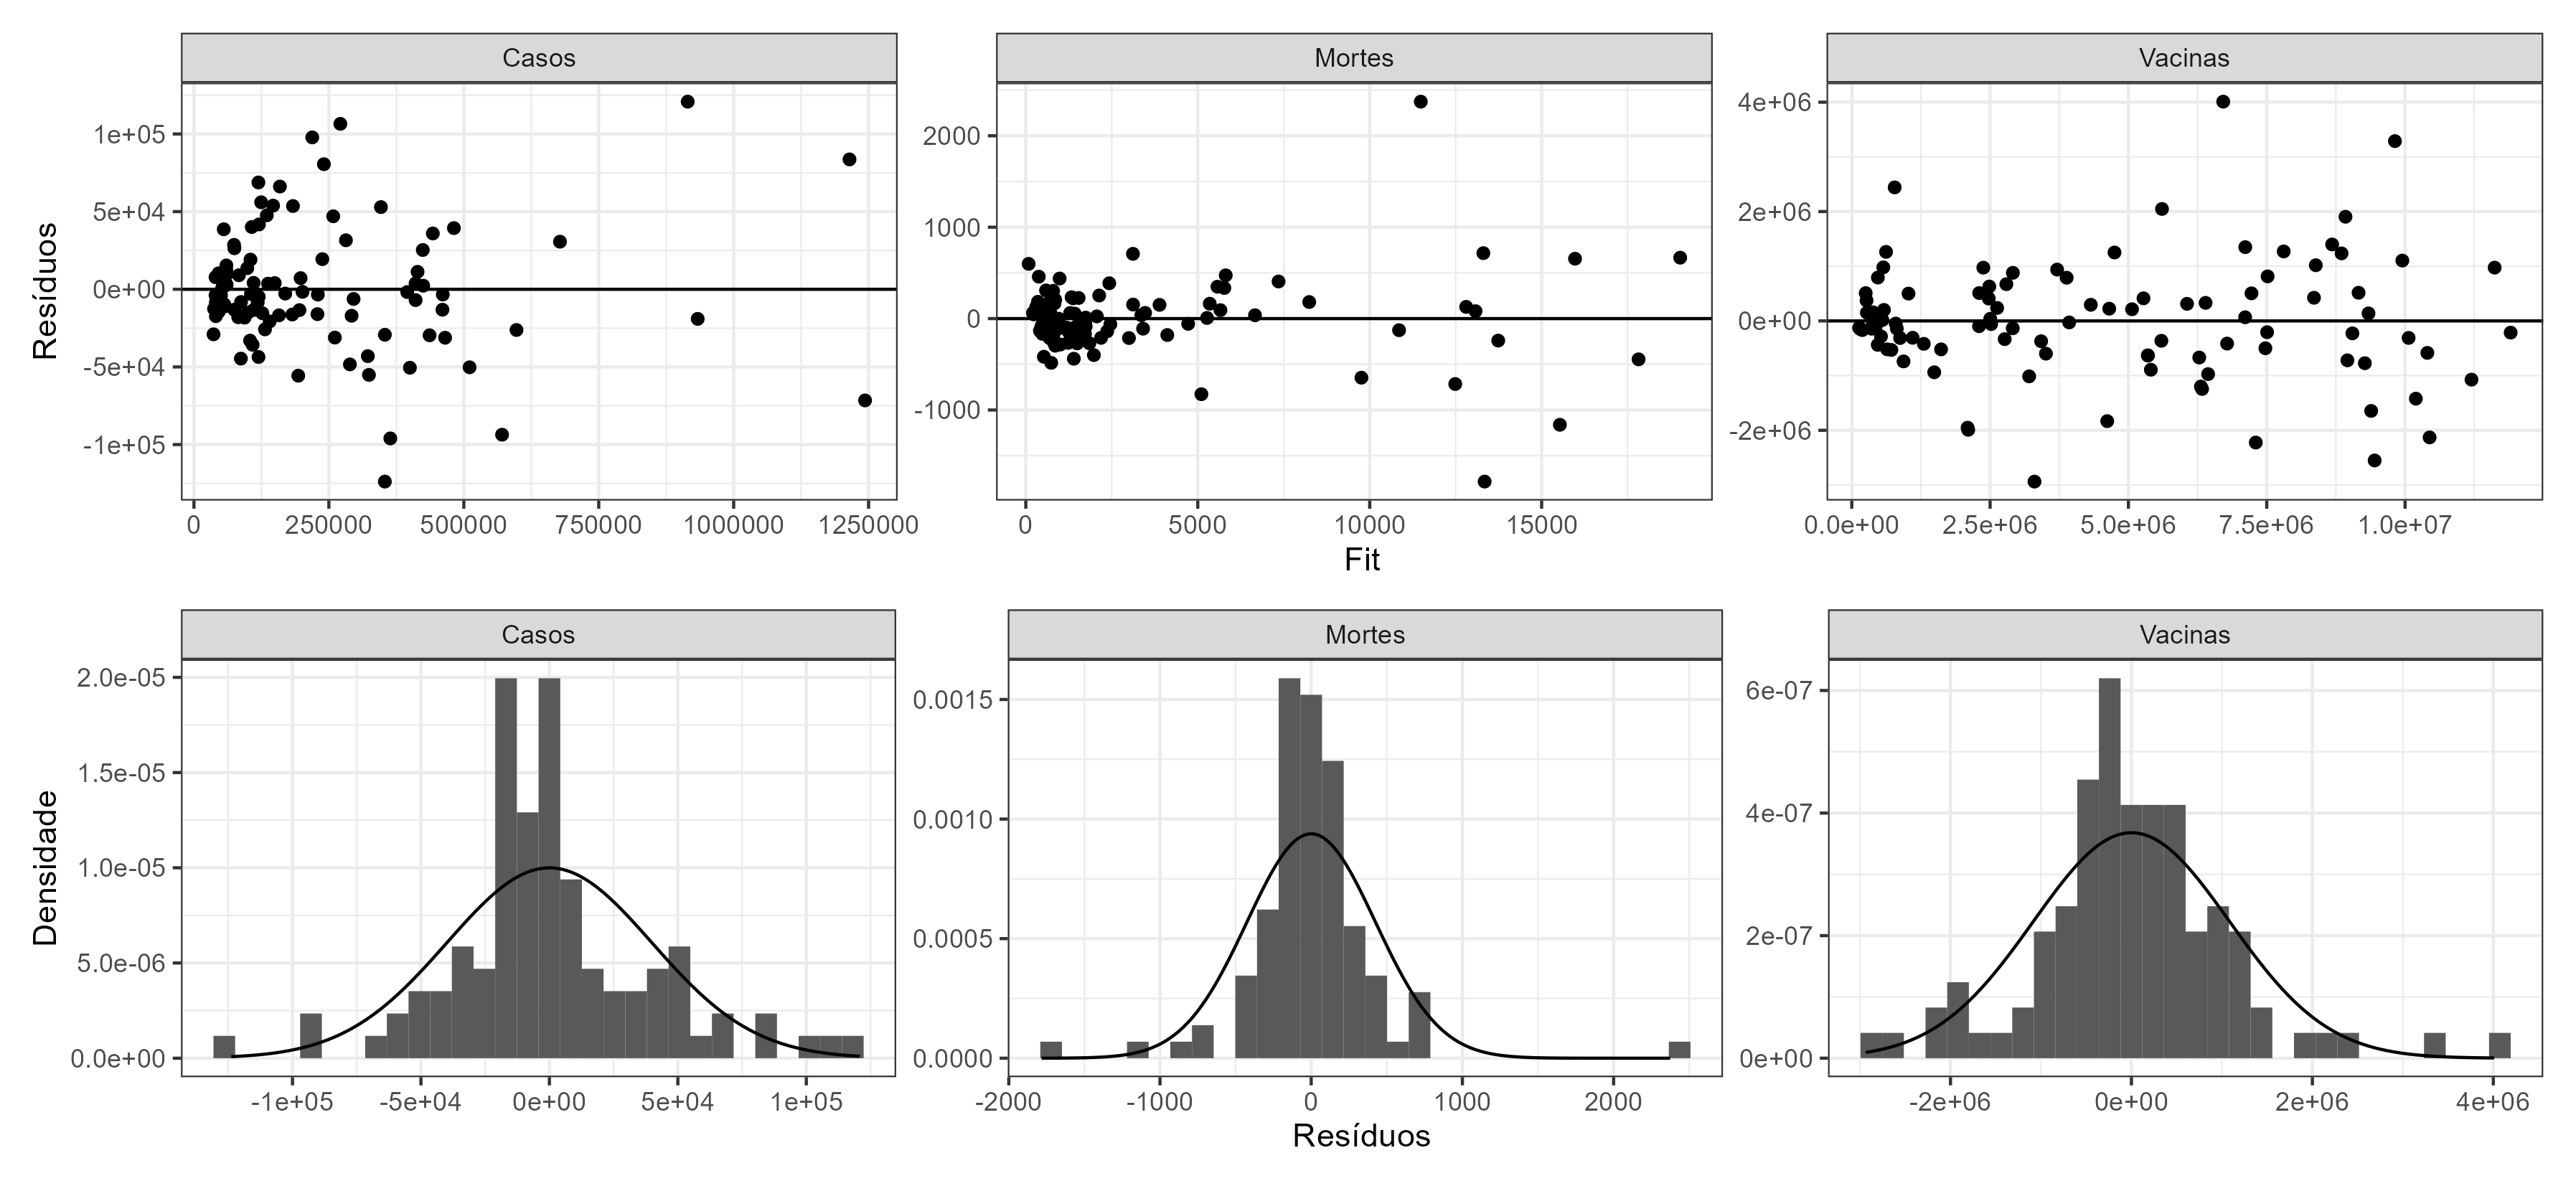
\includegraphics[width = 0.95\textwidth]{Figuras/diag_disp-dist.png}
    \label{fig:varresdist}
\end{figure}

A figura \ref{fig:varresacf} mostra as autocorrelações dos resíduos, indicando dependência temporal insignificante das e entre as variáveis. De fato, o modelo passou teste Portmanteau de autocorrelação dos resíduos (em até $12$ lags) -- estatística do teste de $123,54$, com $126$ graus de liberdade, gerando um p-valor = $0,3215$. Similarmente, o teste Edgerton-Shukur também rejeitou a presença de autocorrelação.

\begin{figure}[H]
    \centering
    \caption{Correlação cruzada e parcial dos resíduos}
    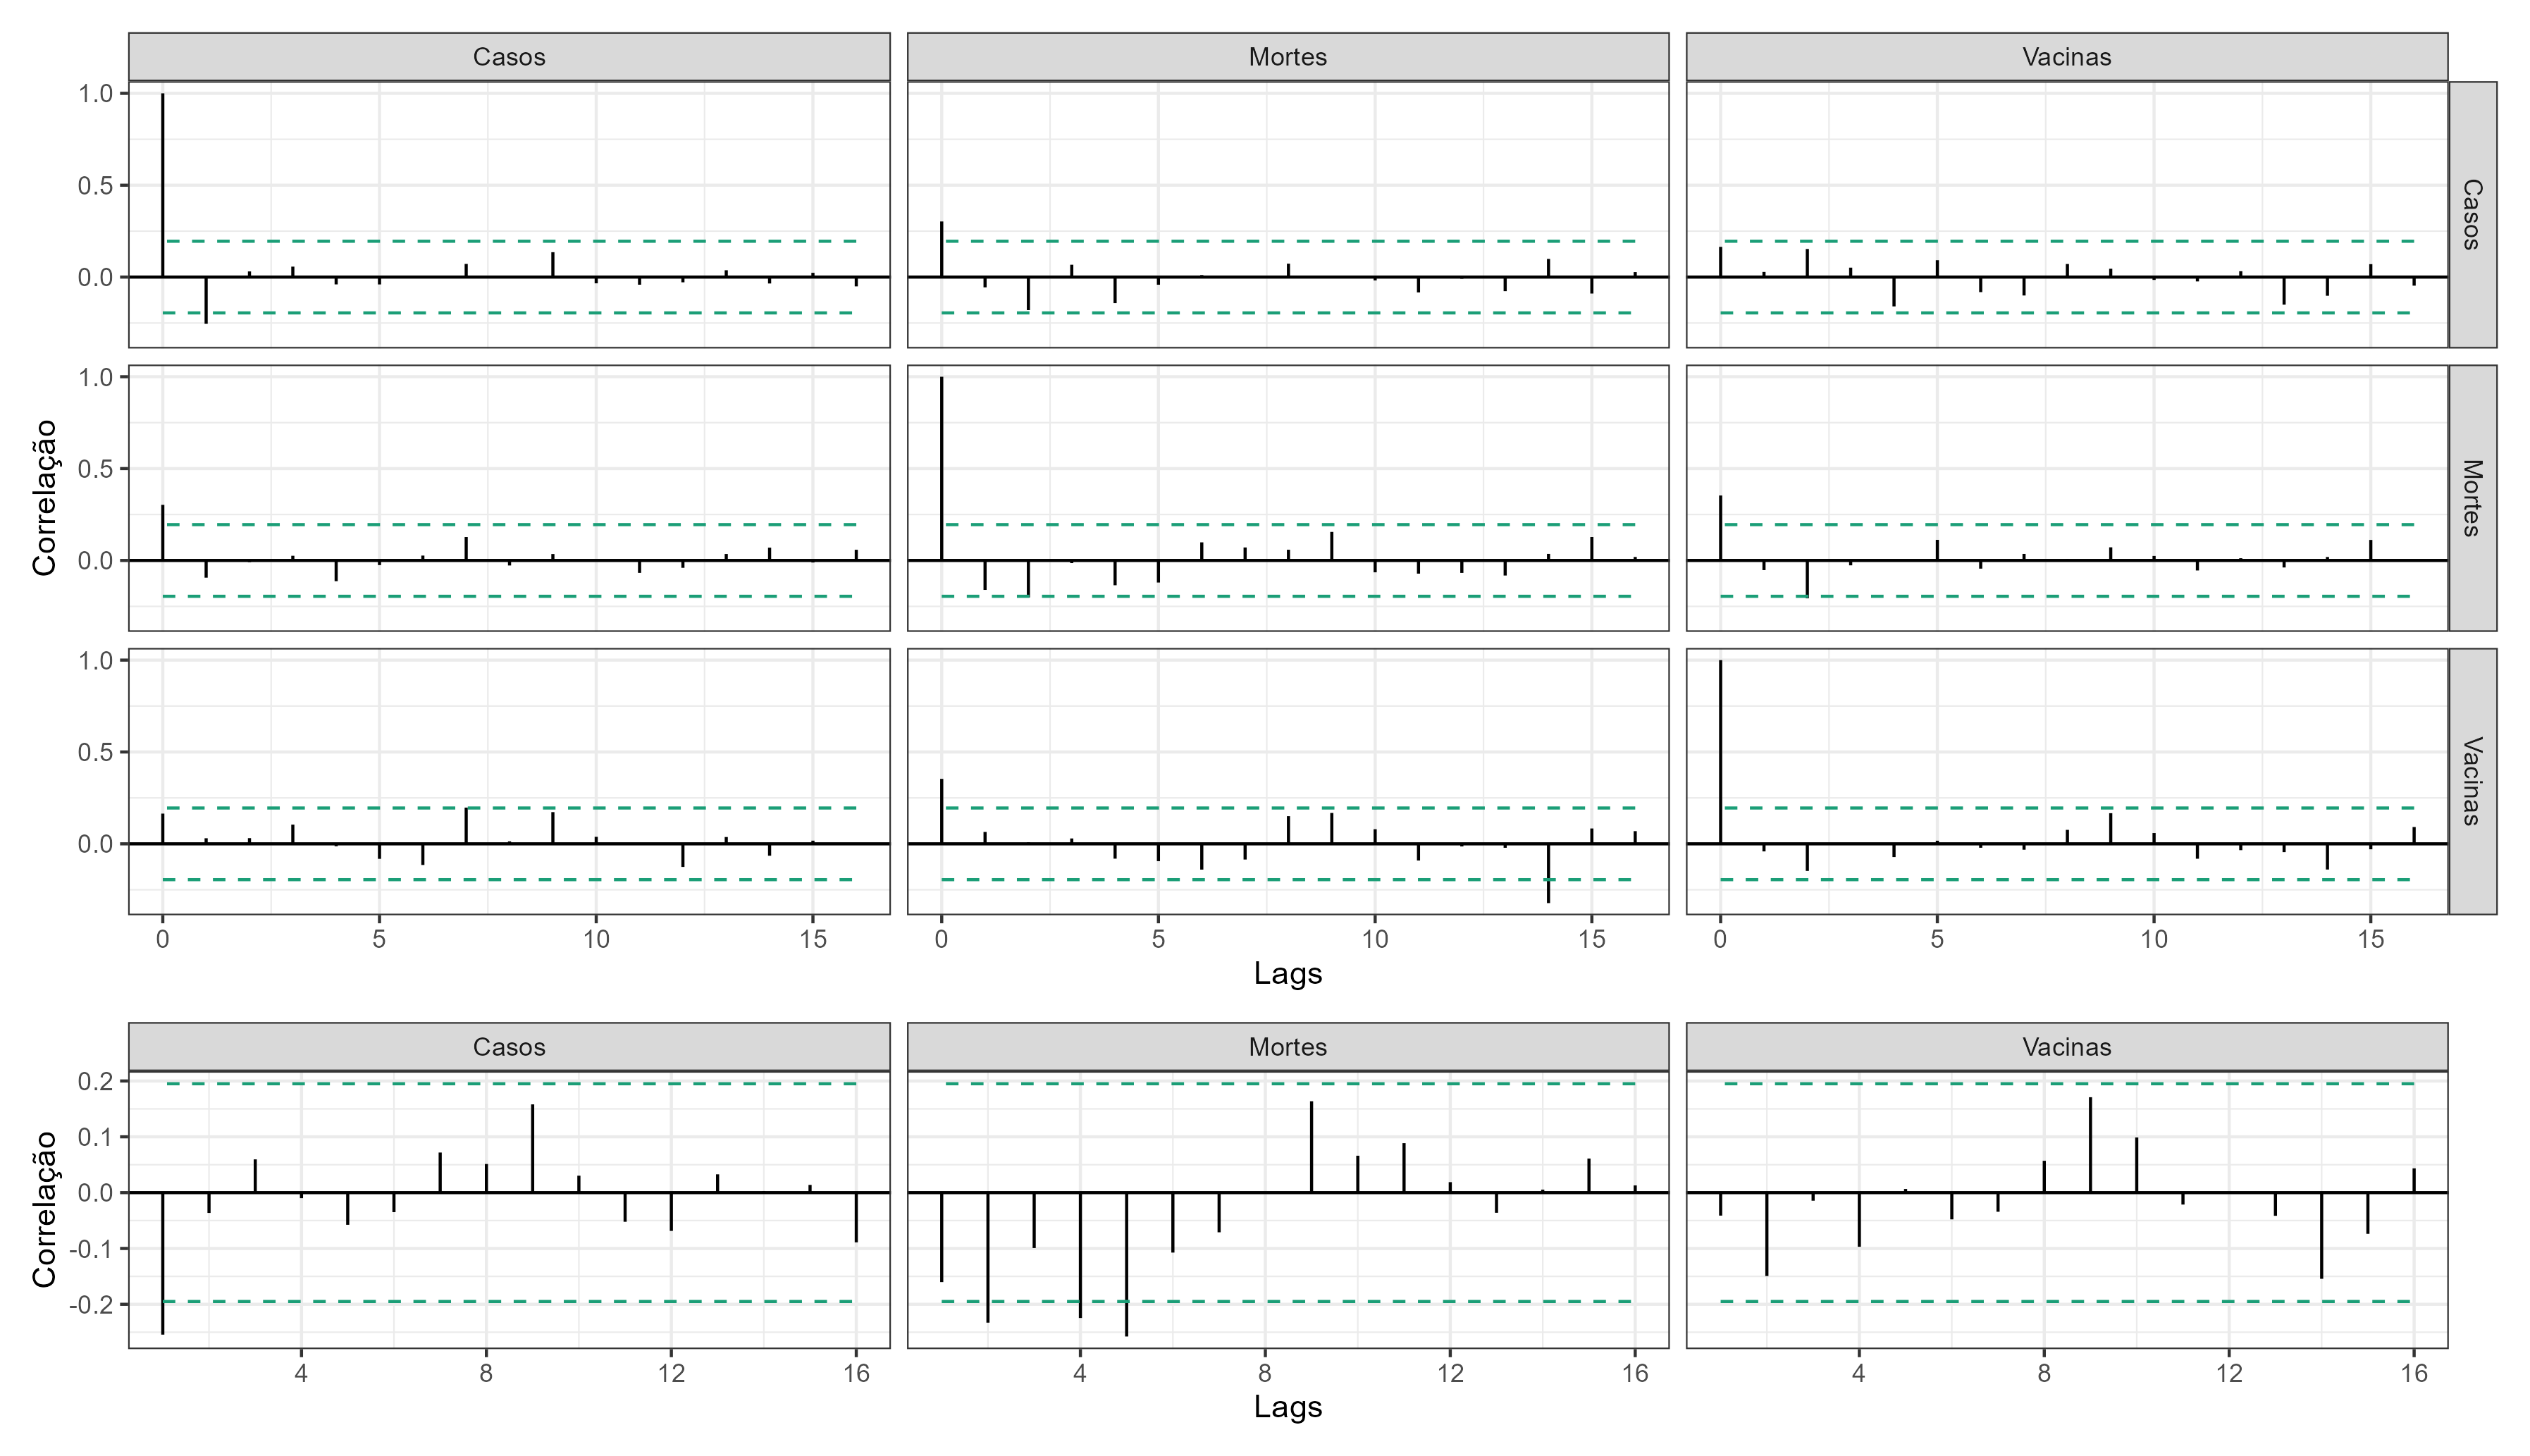
\includegraphics[width = 0.95\textwidth]{Figuras/diag_acf.png}
    \label{fig:varresacf}
\end{figure}

A figura \ref{fig:varstab} mostra a estabilidade dos resíduos do modelo, mais especificamente, o resultado da função ``stability'' do pacote ``vars'' com o método ``CUMSUM-OLS'' no R. Ela indica que alterar a amostra que baseou a estimativa do modelo não altera drasticamente os valores dos coeficientes.

\begin{figure}[H]
    \centering
    \caption{Estabilidade dos resíduos}
    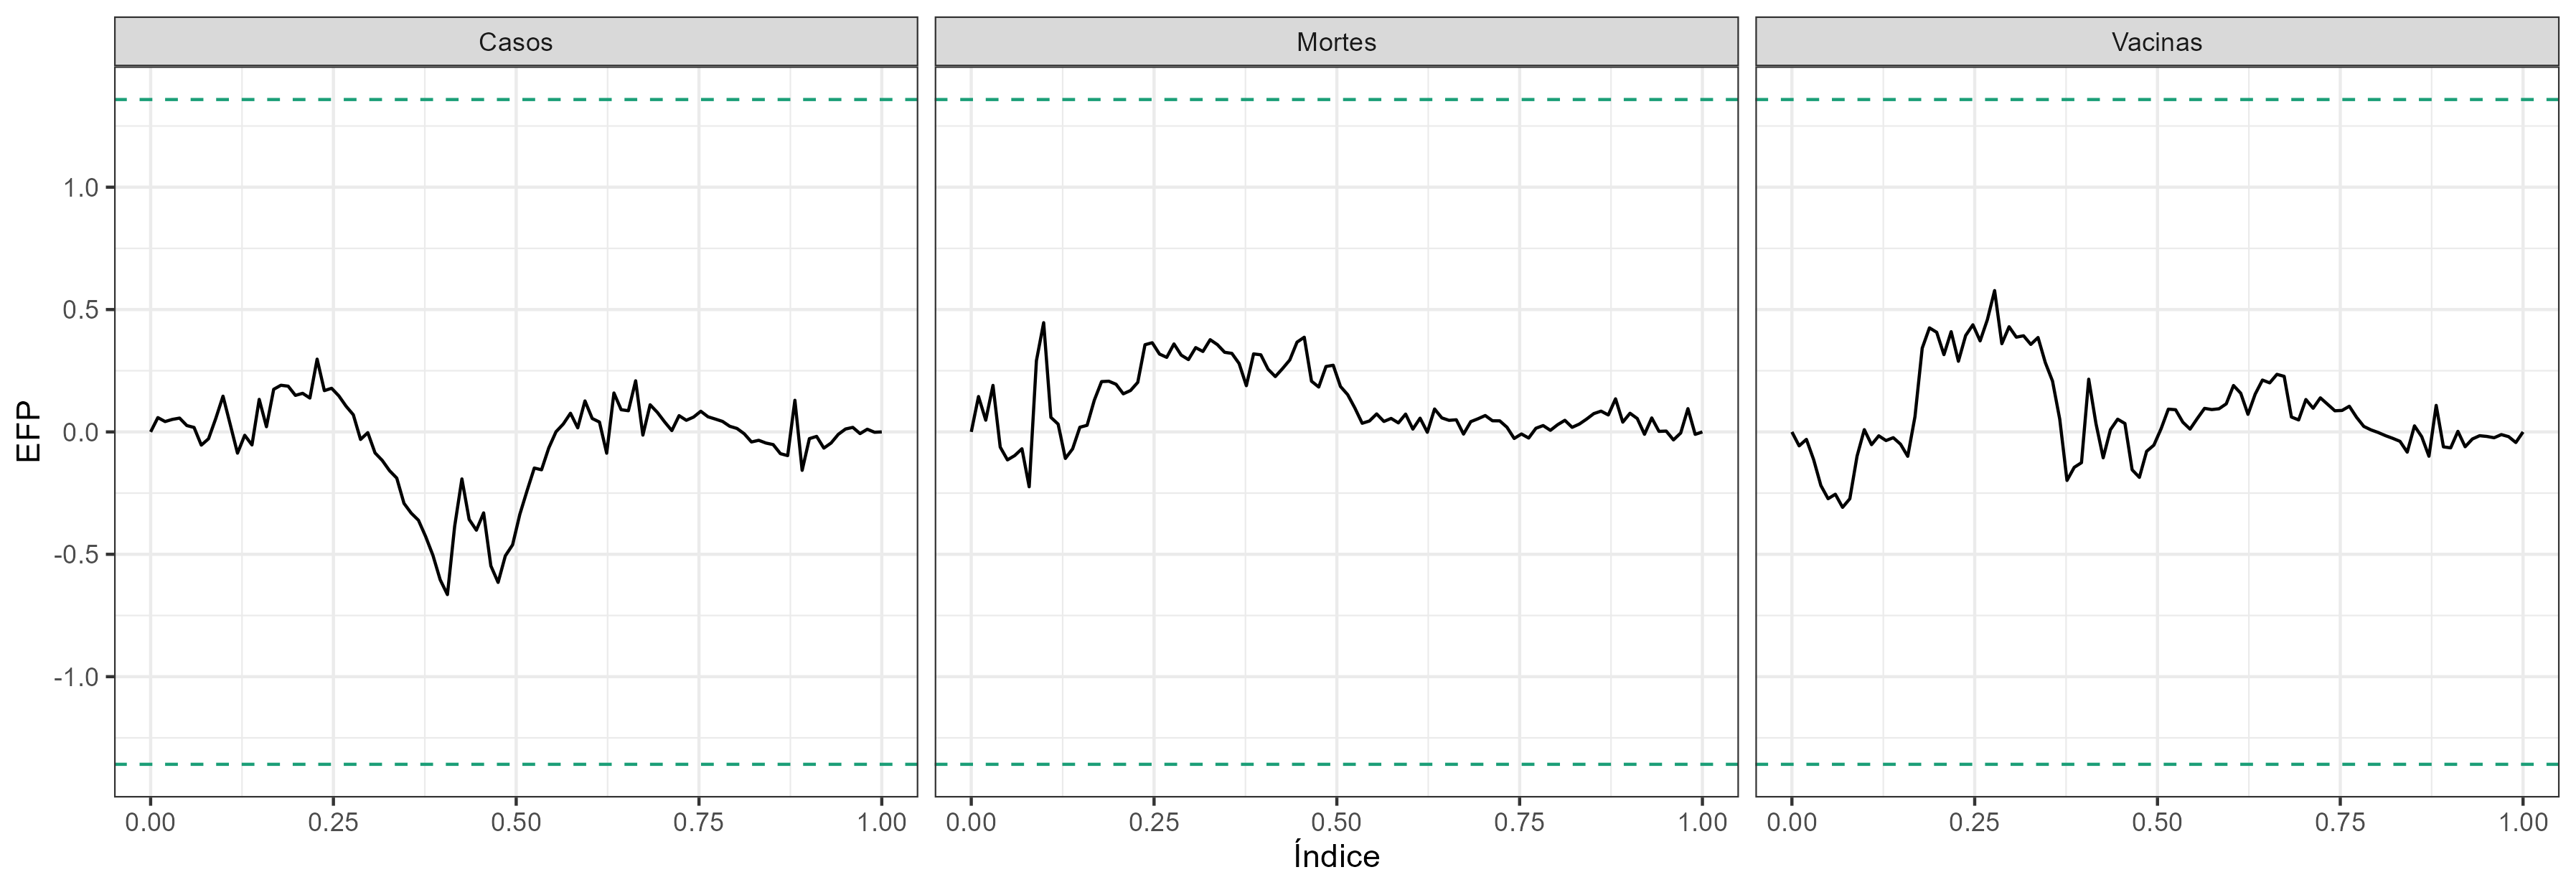
\includegraphics[width = 0.95\textwidth]{Figuras/diag_stab.png}
    \label{fig:varstab}
\end{figure}

Vale atentar que as raízes do VAR são todas menores que 1: $0,909 (<1)$,	$0,886 (<1)$,	$0,886 (<1)$,	$0,754 (<1)$,	$0,754 (<1)$,	$0,563 (<1)$,	$0,563 (<1)$,	$0,522 (<1)$,	$0,522 (<1)$.


\newpage
\chapter{Correlação dos Choques}\label{ap:corres}

As tabelas abaixo apresentam a matriz de correlação dos resíduos do VAR, e ao lado, a matriz de identificação do SVAR (com valores normalizados fora do parênteses), para os modelos \eqref{eq:var1} a \eqref{eq:var5}, respectivamente. Vale notar como a correlação de casos e mortes foi menor nos modelos finais.

\begin{table}[!htbp] \centering 
    %\caption{} 
    \label{} 
  \begin{tabular}{@{\extracolsep{5pt}} ccccc} 
  \\[-1.8ex]\hline 
  \hline \\[-1.8ex] 
  Casos & Mortes &  & Casos.1 & Mortes.1 \\ 
  \hline \\[-1.8ex] 
  1 & 0.915 & \textbar  & 1 (53786) & 0 (0) \\ 
  0.915 & 1 & \textbar  & 2.273 (847) & 1 (372) \\ 
  \hline \\[-1.8ex] 
  \end{tabular} 
\end{table} 
  
\begin{table}[!htbp] \centering 
    %\caption{} 
    \label{} 
  \begin{tabular}{@{\extracolsep{5pt}} ccccc} 
  \\[-1.8ex]\hline 
  \hline \\[-1.8ex] 
  Casos & Mortes &  & Casos.1 & Mortes.1 \\ 
  \hline \\[-1.8ex] 
  1 & 0.467 & \textbar  & 1 (47365) & 0 (0) \\ 
  0.467 & 1 & \textbar  & 0.527 (302) & 1 (572) \\ 
  \hline \\[-1.8ex] 
  \end{tabular} 
\end{table} 
  
\begin{table}[!htbp] \centering 
    %\caption{} 
    \label{} 
  \begin{tabular}{@{\extracolsep{5pt}} ccccccc} 
  \\[-1.8ex]\hline 
  \hline \\[-1.8ex] 
  Casos & Vacinas & Mortes &  & Casos.1 & Vacinas.1 & Mortes.1 \\ 
  \hline \\[-1.8ex] 
  1 & 0.209 & 0.489 & \textbar  & 1 (46188) & 0 (0) & 0 (0) \\ 
  0.209 & 1 & 0.314 & \textbar  & 0.214 (223224) & 1 (1041889) & 0 (0) \\ 
  0.489 & 0.314 & 1 & \textbar  & 0.579 (317) & 0.256 (140) & 1 (547) \\ 
  \hline \\[-1.8ex] 
  \end{tabular} 
\end{table} 
  
\begin{table}[!htbp] \centering 
    %\caption{} 
    \label{} 
  \begin{tabular}{@{\extracolsep{5pt}} ccccc} 
  \\[-1.8ex]\hline 
  \hline \\[-1.8ex] 
  Casos & Mortes &  & Casos.1 & Mortes.1 \\ 
  \hline \\[-1.8ex] 
  1 & 0.308 & \textbar  & 1 (43597) & 0 (0) \\ 
  0.308 & 1 & \textbar  & 0.324 (134) & 1 (412) \\ 
  \hline \\[-1.8ex] 
  \end{tabular} 
\end{table} 
  
\begin{table}[!htbp] \centering 
    %\caption{} 
    \label{} 
  \begin{tabular}{@{\extracolsep{5pt}} ccccccc} 
  \\[-1.8ex]\hline 
  \hline \\[-1.8ex] 
  Casos & Vacinas & Mortes &  & Casos.1 & Vacinas.1 & Mortes.1 \\ 
  \hline \\[-1.8ex] 
  1 & 0.169 & 0.306 & \textbar  & 1 (41258) & 0 (0) & 0 (0) \\ 
  0.169 & 1 & 0.355 & \textbar  & 0.171 (187884) & 1 (1097746) & 0 (0) \\ 
  0.306 & 0.355 & 1 & \textbar  & 0.34 (134) & 0.342 (134) & 1 (393) \\ 
  \hline \\[-1.8ex] 
  \end{tabular} 
\end{table} 



\newpage
\chapter{IRF's Individuais}\label{ap:single}

Como foi explicado, a identificação dos choques não é muito robusta, e existem variáveis omitidas no modelo, de modo que a análise das IRF's individualmente não é prioritária. De qualquer forma, pode-se vê-las na figura \ref{fig:apirf}. De fato, contra o que as análises mais robustas indicam, o efeito da vacina em casos e mortes não se mostra negativo.

\begin{figure}[H]
    \centering
    \caption{IRF's do modelo (5)}
    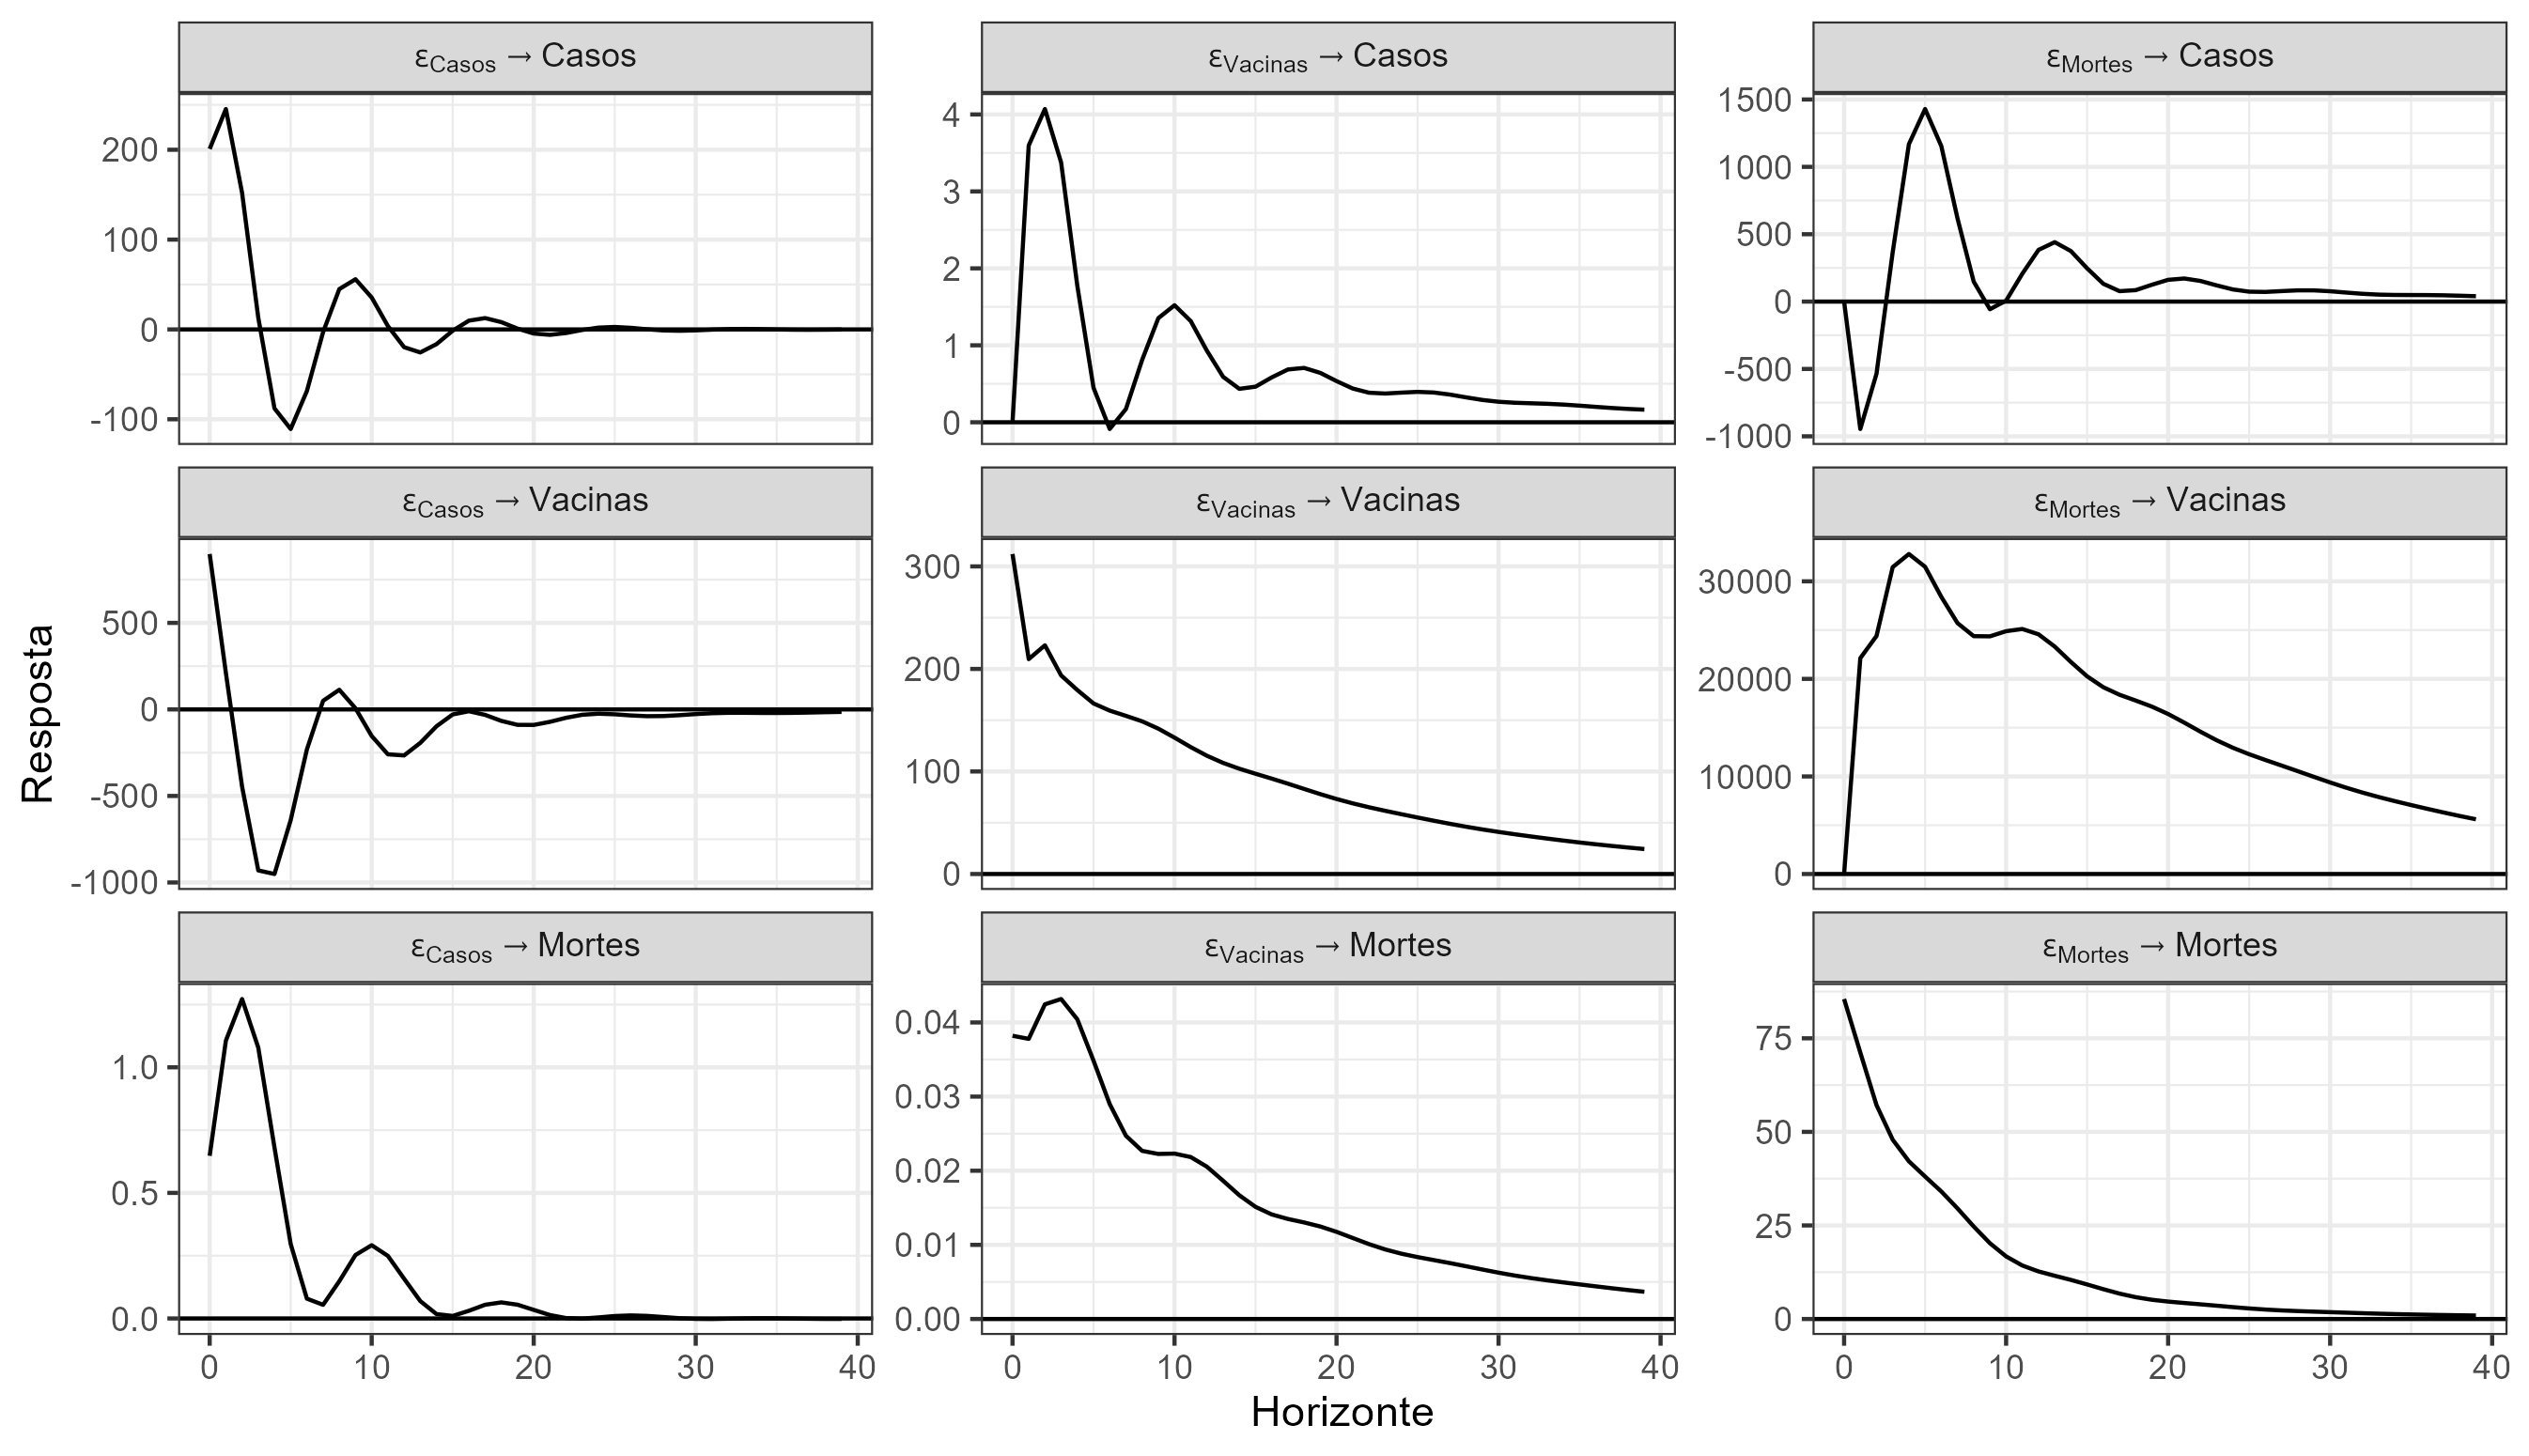
\includegraphics[width = 0.95\textwidth]{Figuras/ap_irfs.png}
    \label{fig:apirf}
\end{figure}

Outro possível objeto de interesse são as \textit{Forecast Error Variance Decomposition} (FEVD), que indicam a fração da contribuição de cada variável para a variância da previsão de cada equação. A figura \ref{fig:apfevd}. As vacinas parecem explicar uma maior porcentagem da variância nas mortes do que dos casos, embora não seja o \textit{driver} majoritário em nenhum dos dois.

\begin{figure}[H]
    \centering
    \caption{FEVD's do modelo (5)}
    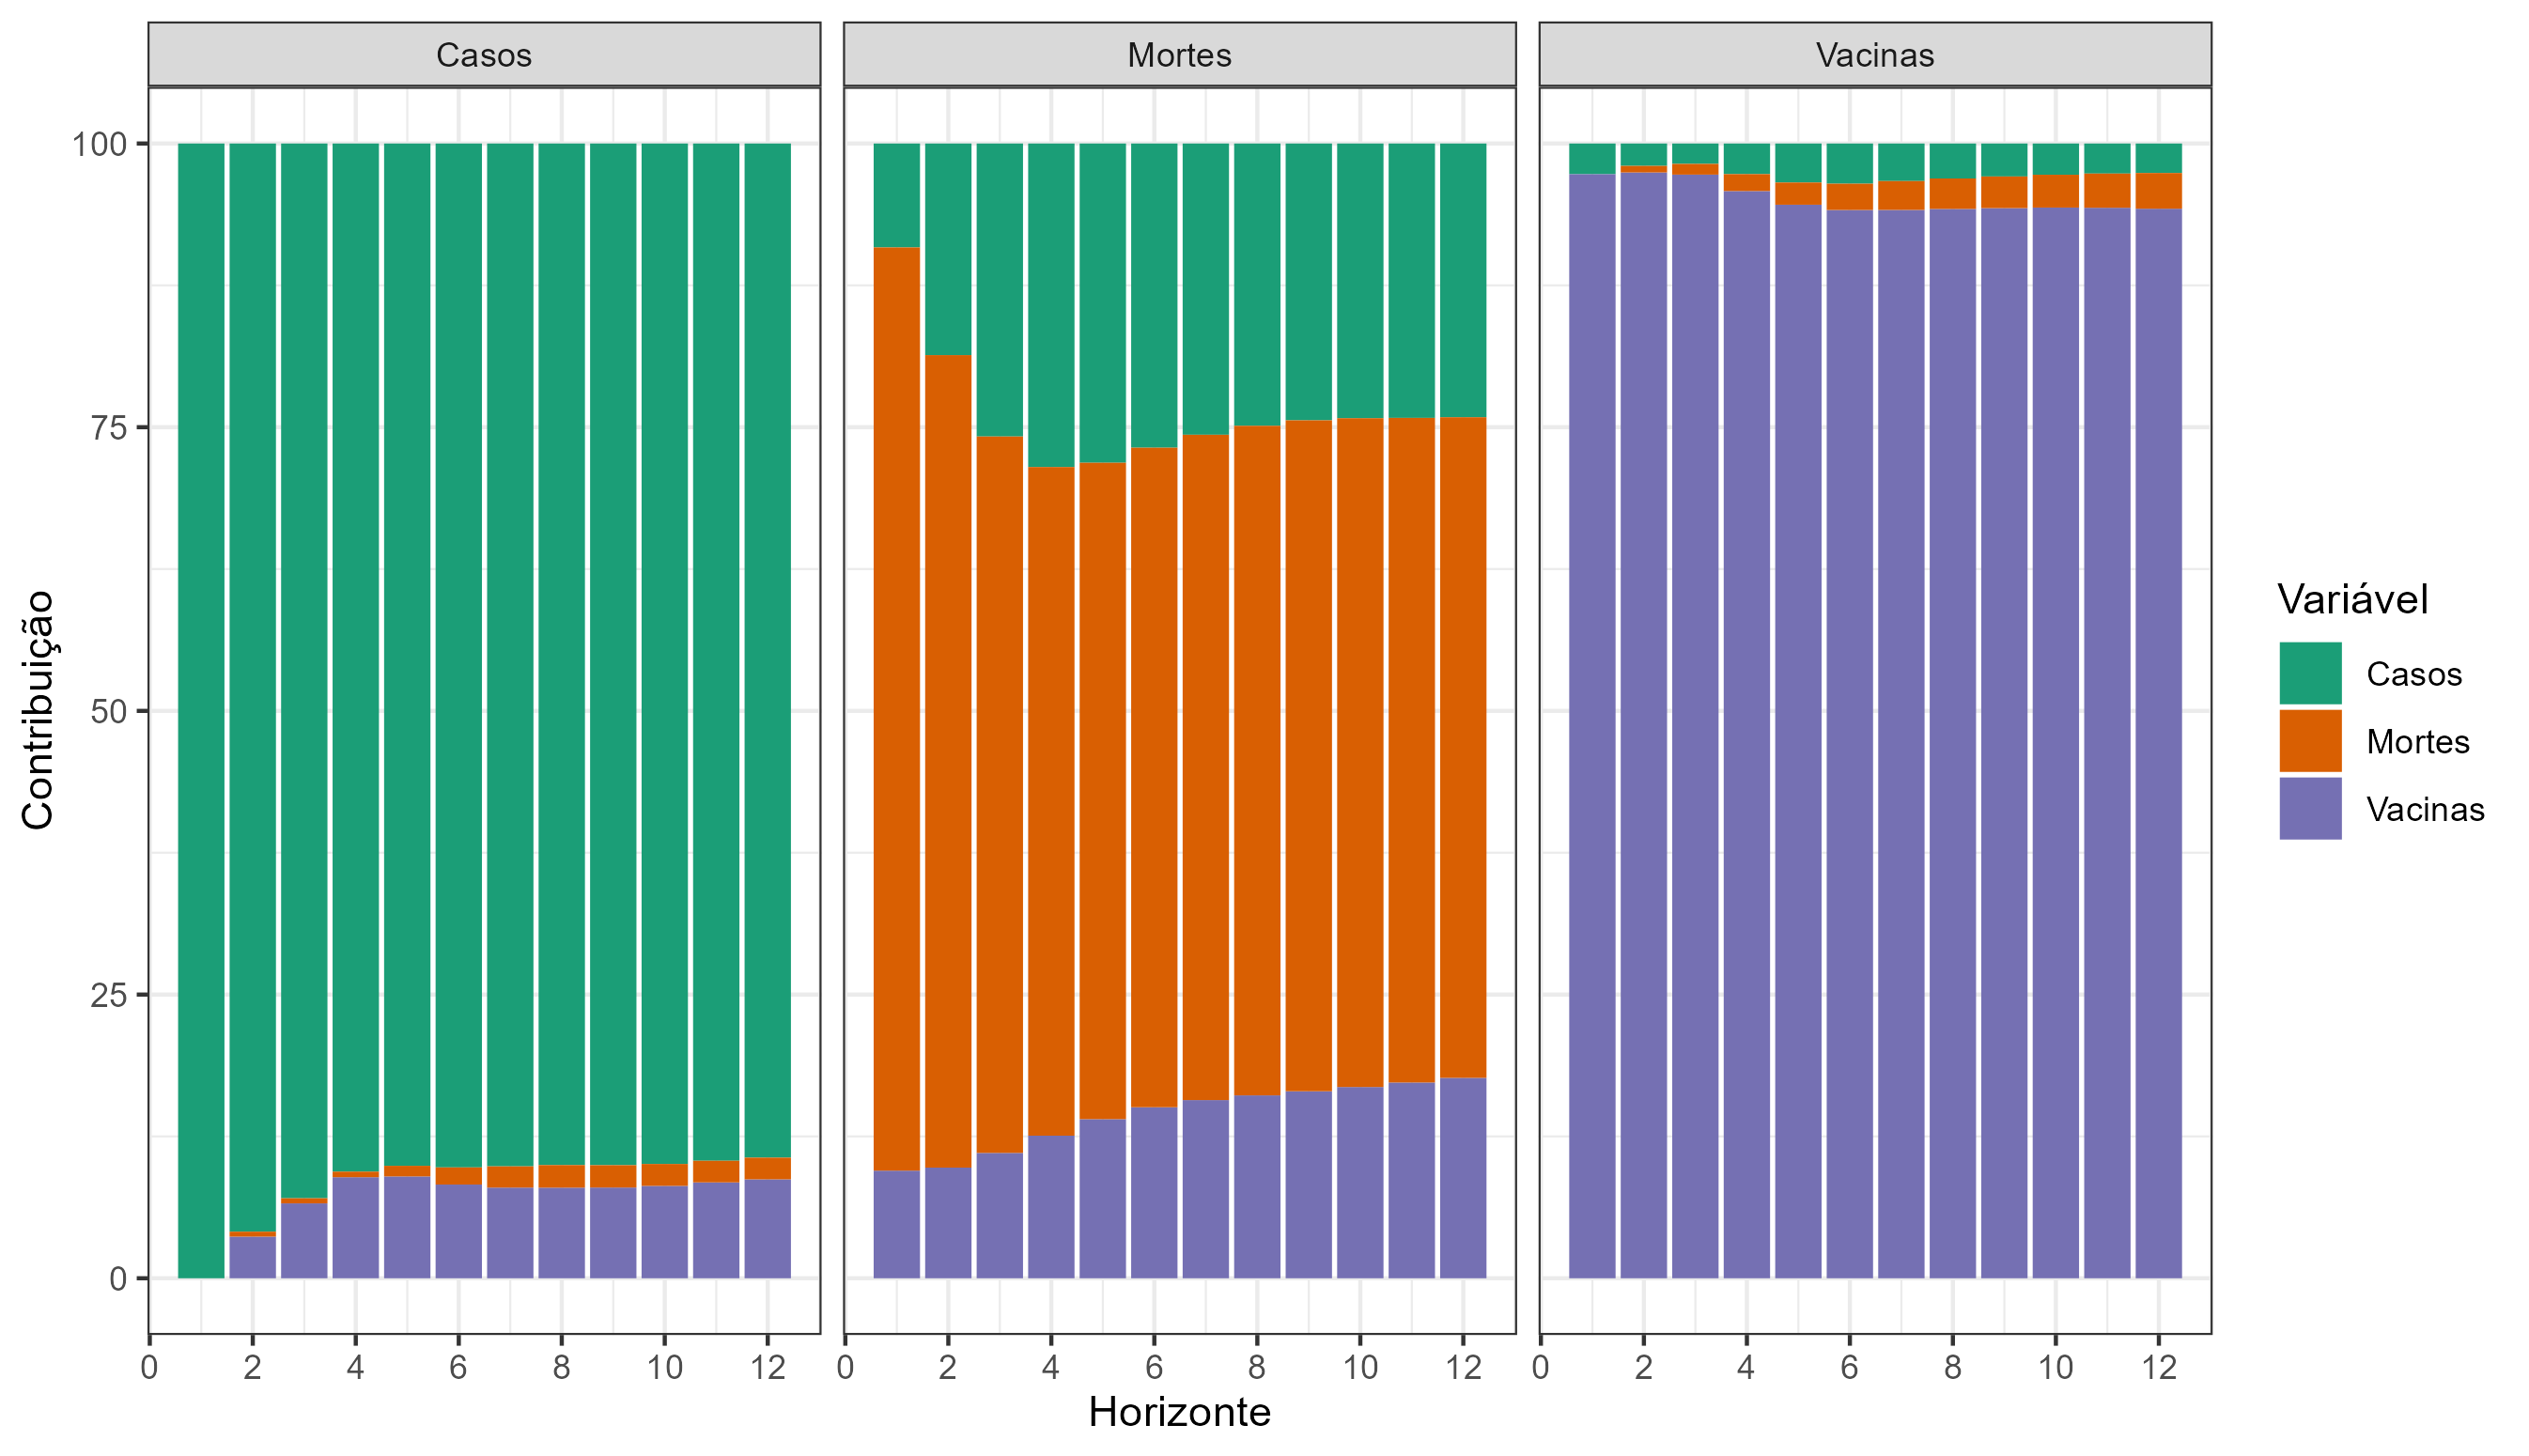
\includegraphics[width = 0.95\textwidth]{Figuras/ap_fevd.png}
    \label{fig:apfevd}
\end{figure}

\newpage %página extra para resolver bug de remoção dá última página


\end{apendicesenv}

\end{document}
